% Written on jeu. 19 juin 2025 12:51:09 CEST
% by Jean-Baptiste Caillau - Université Côte d'Azur, CNRS, Inria, LJAD
% todo:
\documentclass[9pt]{beamer}
\usepackage[applemac]{inputenc}   
\usepackage[T1]{fontenc}
\usepackage{lmodern}
\usepackage{graphicx}
%\usepackage{graphicx,psfrag,epsfig}
%\usepackage[english]{babel}
%\usepackage{subfigure}
\usepackage{amsmath, amsfonts, amssymb, amsthm}
\usepackage{hyperref} 
%\usepackage{ccaption}
\hypersetup{colorlinks = true, urlcolor = blue, bookmarksopen = true}
\usepackage{array}
\usepackage{color}
\usepackage{mathrsfs}
\usepackage{wasysym}
\usepackage{algorithm,algorithmic}
\usepackage{fancybox}
\usepackage{mathptmx}
\setbeamertemplate{navigation symbols}{}
\setbeamertemplate{theorems}[numbered]
%\addtobeamertemplate{footline}{\insertframenumber / \inserttotalframenumber}
%
\def\R{\mathbf{R}}
\def\B{\mathbf{B}}
\def\SS{\mathbf{S}}
\def\Z{\mathbf{Z}}
\def\N{\mathbf{N}}
\def\W{\text{W}}
\def\L{L}
\def\C{\mathbf{C}}
\def\D{\mathbf{D}}
\def\P{\mathbf{P}}
\def\V{\mathbf{V}}
\def\CC{\mathscr{C}}
\def\LL{\mathscr{L}}
\def\DD{\mathscr{D}}
\def\ee{\mathbf{e}}
\def\H{\text{H}}
\def\arcsh{\text{arcsh}}
\def\arctan{\text{arctan}}
\def\ch{\text{ch}}
\def\sh{\text{sh}}
\def\cn{\text{cn}}
\def\sn{\text{sn}}
\def\dn{\text{dn}}
\def\codim{\text{codim}}
\def\Im{\text{Im}}
\def\Sp{\text{Sp}}
\def\cst{\text{cst}}
\def\Tmax{T_\text{max}}
\def\iy{\infty}
\def\t{\ \!^t\!}
\def\veps{\varepsilon}
\renewcommand\Re{\text{Re}}
\renewcommand\d{\text{d}}
\renewcommand\vec{\overrightarrow}
\renewcommand\bar{\overline}
\def\vphi{\varphi}
\def\wtilde{\widetilde}
\def\co{\text{co}}
\def\cl{\text{cl}}
\def\tr{\text{tr}}
\def\intr{\text{int}}
\def\cut{\text{cut}}
\def\cone{\text{cone}}
\def\Lie{\text{Lie}}
\def\GL{\text{GL}}
\def\SL{SL}
\def\id{\text{id}}
\def\ad{\text{ad}}
\def\Ad{\text{Ad}}
\def\Vec{\text{Vec}}
\def\Ker{\text{Ker}}
\def\rank{\text{rank}}
\def\rang{\text{rang}}
\def\Cut{\text{Cut}}
\def\Diff{\text{Diff}}
\def\Der{\text{Der}}
\def\xp{\vec{\exp}}
\def\wdg{\wedge}
\def\gat{\tilde{\gamma}}
\def\ie{\emph{i.e.}}
\def\cf{\emph{cf.}}
\def\eg{\emph{e.g.}}
\def\apriori{\emph{a priori}}
\def\etc{\emph{etc.}}
\def\wrt{\emph{w.r.t.}}
\def\resp{\emph{resp.}}
\def\sth{\emph{s.t.}}
\def\noi{\noindent}
\def\bs{\backslash}
\newcommand{\lb}[2]{[#1,#2]}
\def\Vect{\text{Vect}}
\def\span{\text{span}}
\def\sinhc{\text{sinhc}}
\def\la{\langle}
\def\ra{\rangle}
\def\tcut{t_\text{cut}}
\def\umax{u_\text{max}}
\def\cotcot{\texttt{cotcot}}
\def\fortran{\textsl{Fortran}}
\def\adifor{\textsl{Adifor}}
\def\netlib{\textsl{Netlib}}
\def\matlab{\textsl{Matlab}}
\def\Fmax{F_\text{max}}
\def\pr{{p_r}}
\def\For{F_\text{or}}
\def\uor{u_\text{or}}
\def\Isp{I_\text{sp}}
\newcommand{\frp}[2]{\frac{\partial #1}{\partial #2}}
\newcommand{\frpp}[2]{\partial #1/\partial #2}
\renewcommand{\refname}{}
\definecolor{blue1}{RGB}{0,51,153}
\definecolor{green1}{RGB}{0,102,51}
\definecolor{yellow1}{RGB}{255,153,0}
\newcommand{\empha}[1]{\textcolor{blue1}{#1}}
\newcommand{\emphb}[1]{\textcolor{yellow1}{#1}}
\newcommand{\emphc}[1]{\textcolor{green1}{#1}}

\title{\Large \bf De la g\'eom\'etrie \`a la pelle (et r\'eciproquement)}
\author{\textbf{Jean-Baptiste~Caillau}\\
Universit\'e C\^ote d'Azur, CNRS, Inria, LJAD}

\date{\textbf{\emphc{Lyc\'ee Massena}}, Juin 2025}

\begin{document}

% Title
\frame{\titlepage
\begin{center}

\includegraphics[height=1.2cm]{pelle}\\

\includegraphics[height=0.9cm]{logo-uca} \hspace{.1cm}

\includegraphics[height=0.9cm]{cnrs}

\includegraphics[height=0.9cm]{inria}
%
\includegraphics[height=0.9cm]{france-2030}
\end{center}}

% Lecture du bol de caf\'e
\begin{frame}
\frametitle{\bf Lecture du bol de caf\'e}
 
\centering 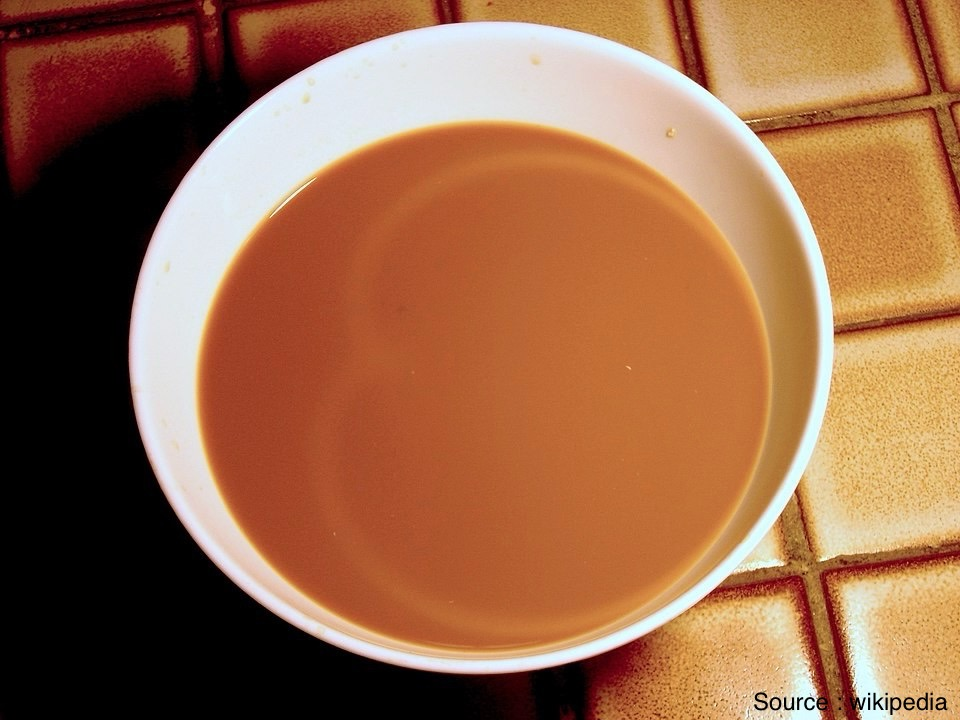
\includegraphics[height=6.0cm]{bol}

\end{frame}

% Catacaustique sur un disque \`a une deux faces
\begin{frame}
\frametitle{\bf Catacaustique sur un disque \`a deux faces}
 
\centering 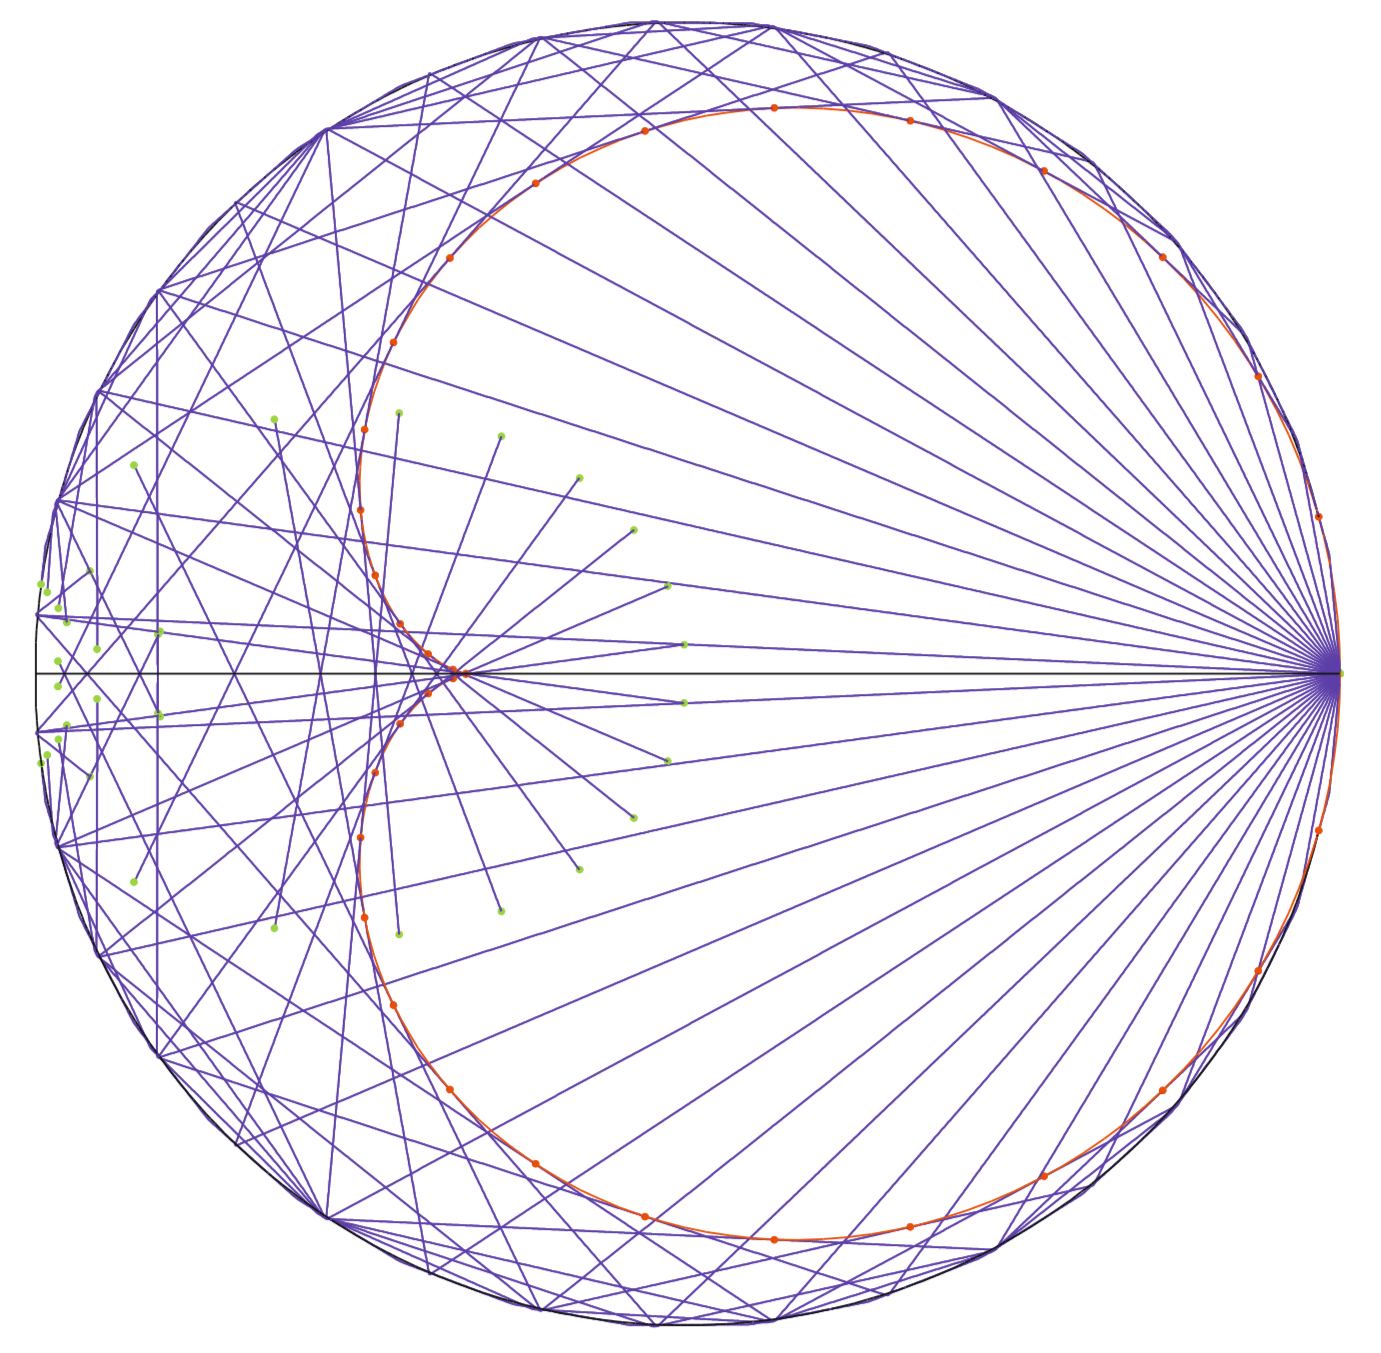
\includegraphics[height=6.0cm]{cata}

\end{frame}

% Les quatre travaux de Gaspard
\begin{frame}
\frametitle{\bf Les quatre travaux de Gaspard}

\centering 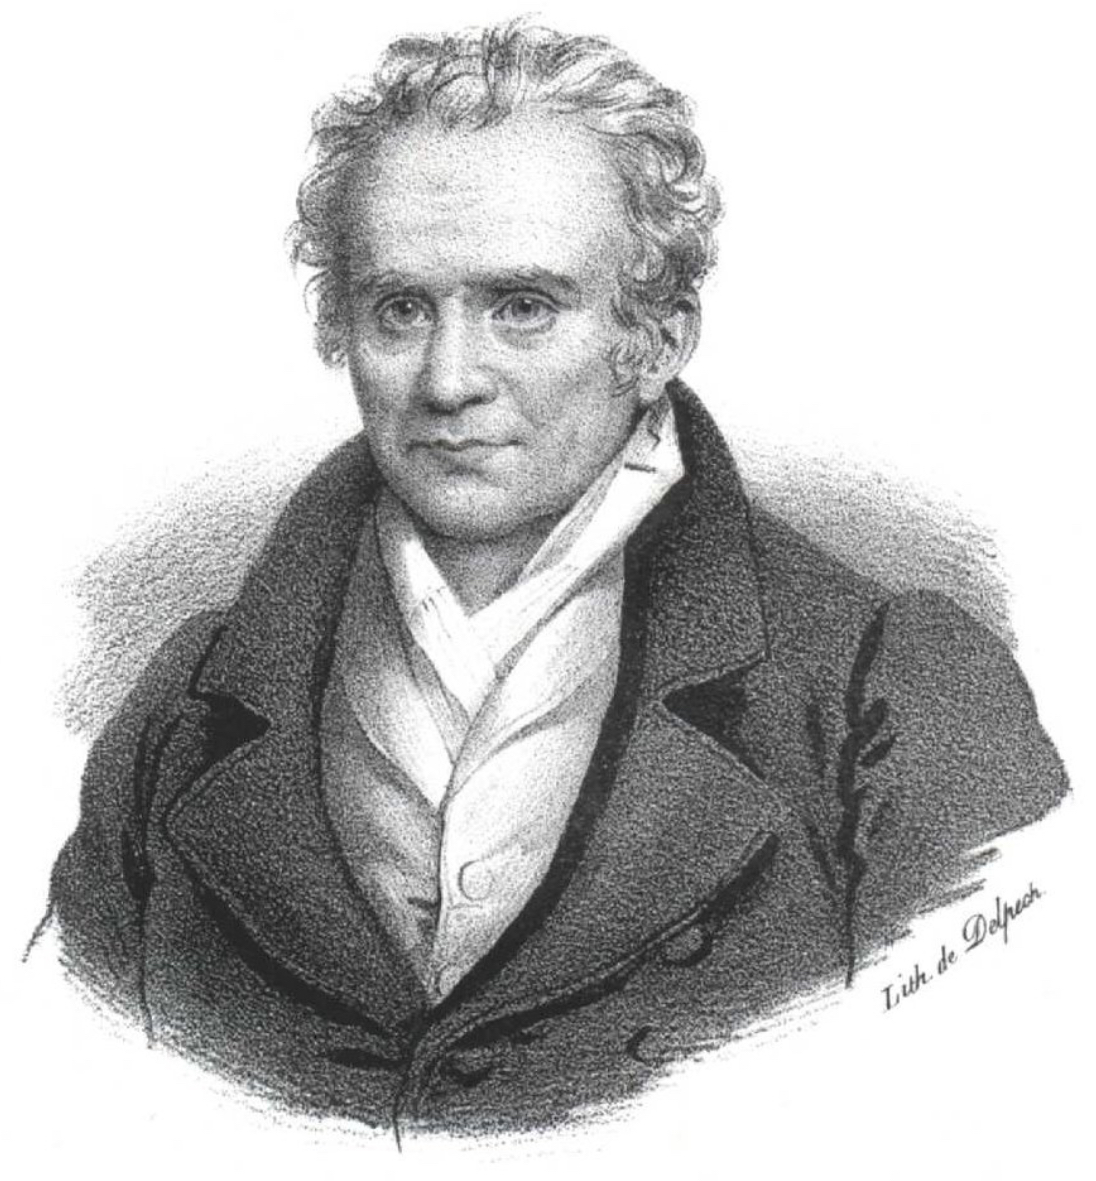
\includegraphics[height=2.0cm]{monge}

\begin{itemize}
  \item Gaspard Monge, 1746--1818 (natif de Beaune, Bourgogne)
  \item Autres scientifiques de son temps : L. Euler (1707-1783), C.~F. Gauss (1777-1855)
  \item Enseignant (dessinateur, assistant pr\'eparateur) \`a l'\'ecole du G\'enie de M\'ezi\`eres
  \item Engagement politique pendant la R\'evolution fran\c caise
  \item Fondateur de l'\'Ecole Polytechnique (1794)
  \item Engagement politique aupr\`es de Napol\'eon Bonaparte (campagne d'\'Egypte)
  \item Disgr\^ace \`a la Restauration
  \item Exemples de travaux : "Machines diverses", "Sur le froid, "Calcul des chances", "Machine \`a remonter les bateaux", "Moulins \`a sucre", "Th\'eorie des torrents et des rivi\`eres et moyen d'emp\^echer leurs ravages"
\end{itemize}
 
\end{frame}

% 1. D\'efilement d'une place forte
\begin{frame}
\frametitle{\bf 1. D\'efilement d'une place forte}
 
\centering 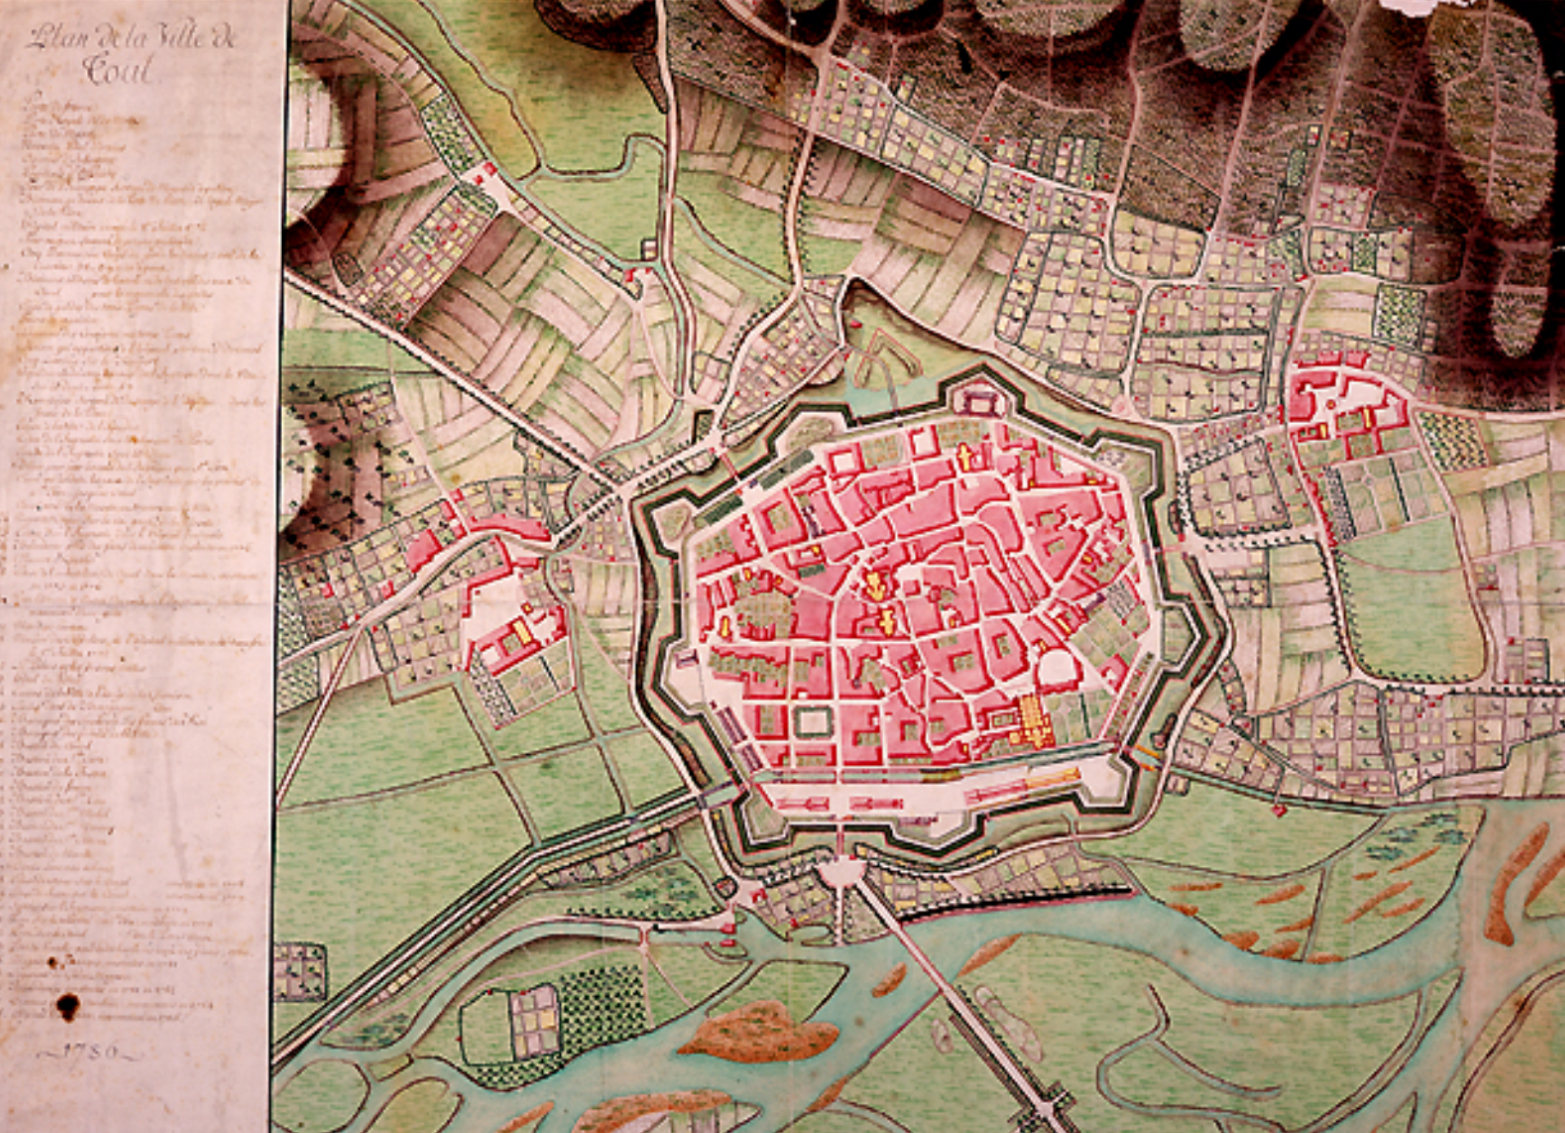
\includegraphics[height=4.0cm]{defil1}

\centering 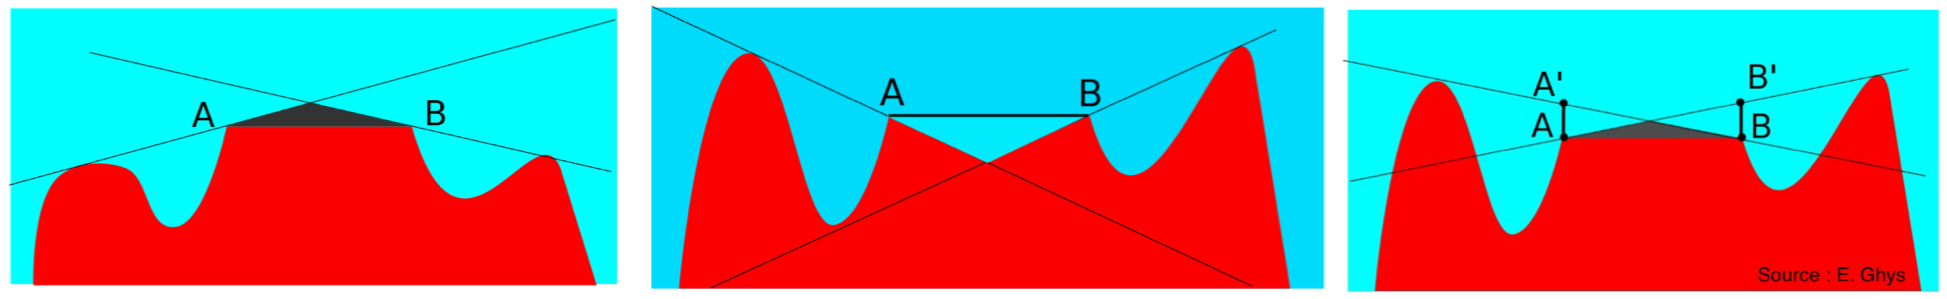
\includegraphics[height=1.7cm]{defil2}

\end{frame}

% 2. Coupe des pierres
\begin{frame}
\frametitle{\bf 2. Coupe des pierres}
 
\centering 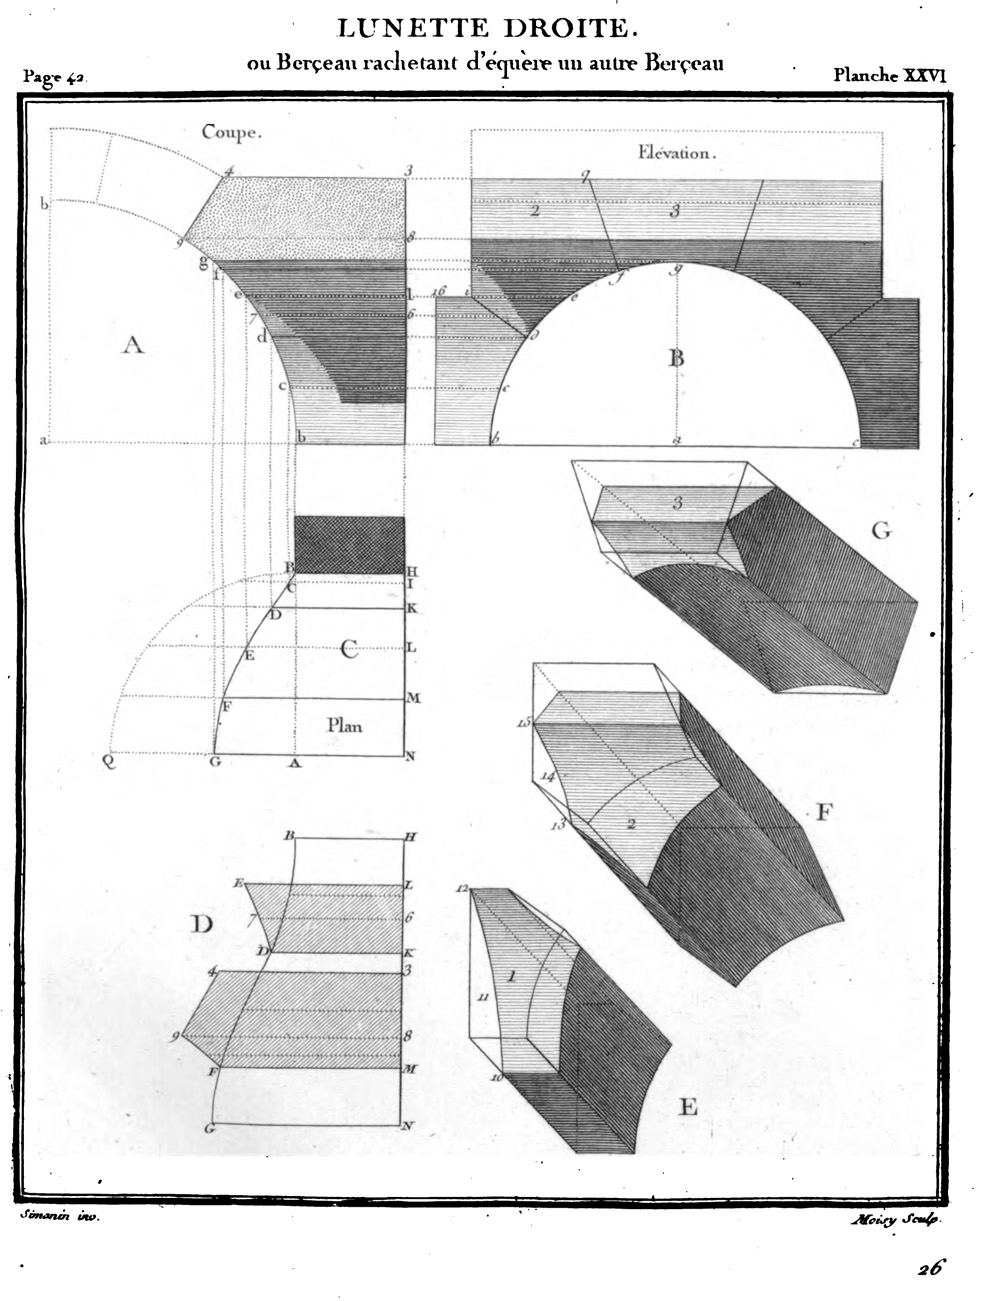
\includegraphics[height=8.0cm]{pierres}

\end{frame}

% 3. Ombres port\'ees
\begin{frame}
\frametitle{\bf 3. Ombres port\'ees}
 
\centering 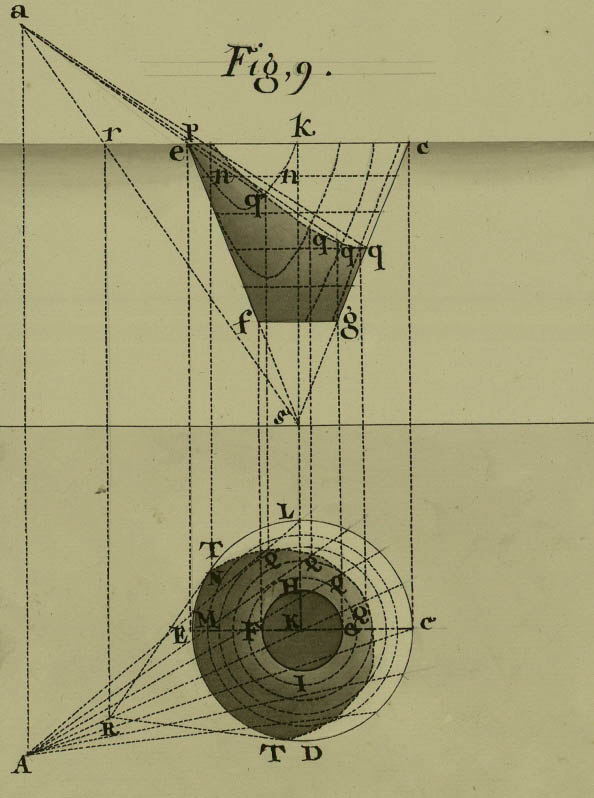
\includegraphics[height=8.0cm]{ombres}

\end{frame}

% 4. D\'eblais et remblais
\begin{frame}
\frametitle{\bf 4. D\'eblais et remblais}
 
\centering 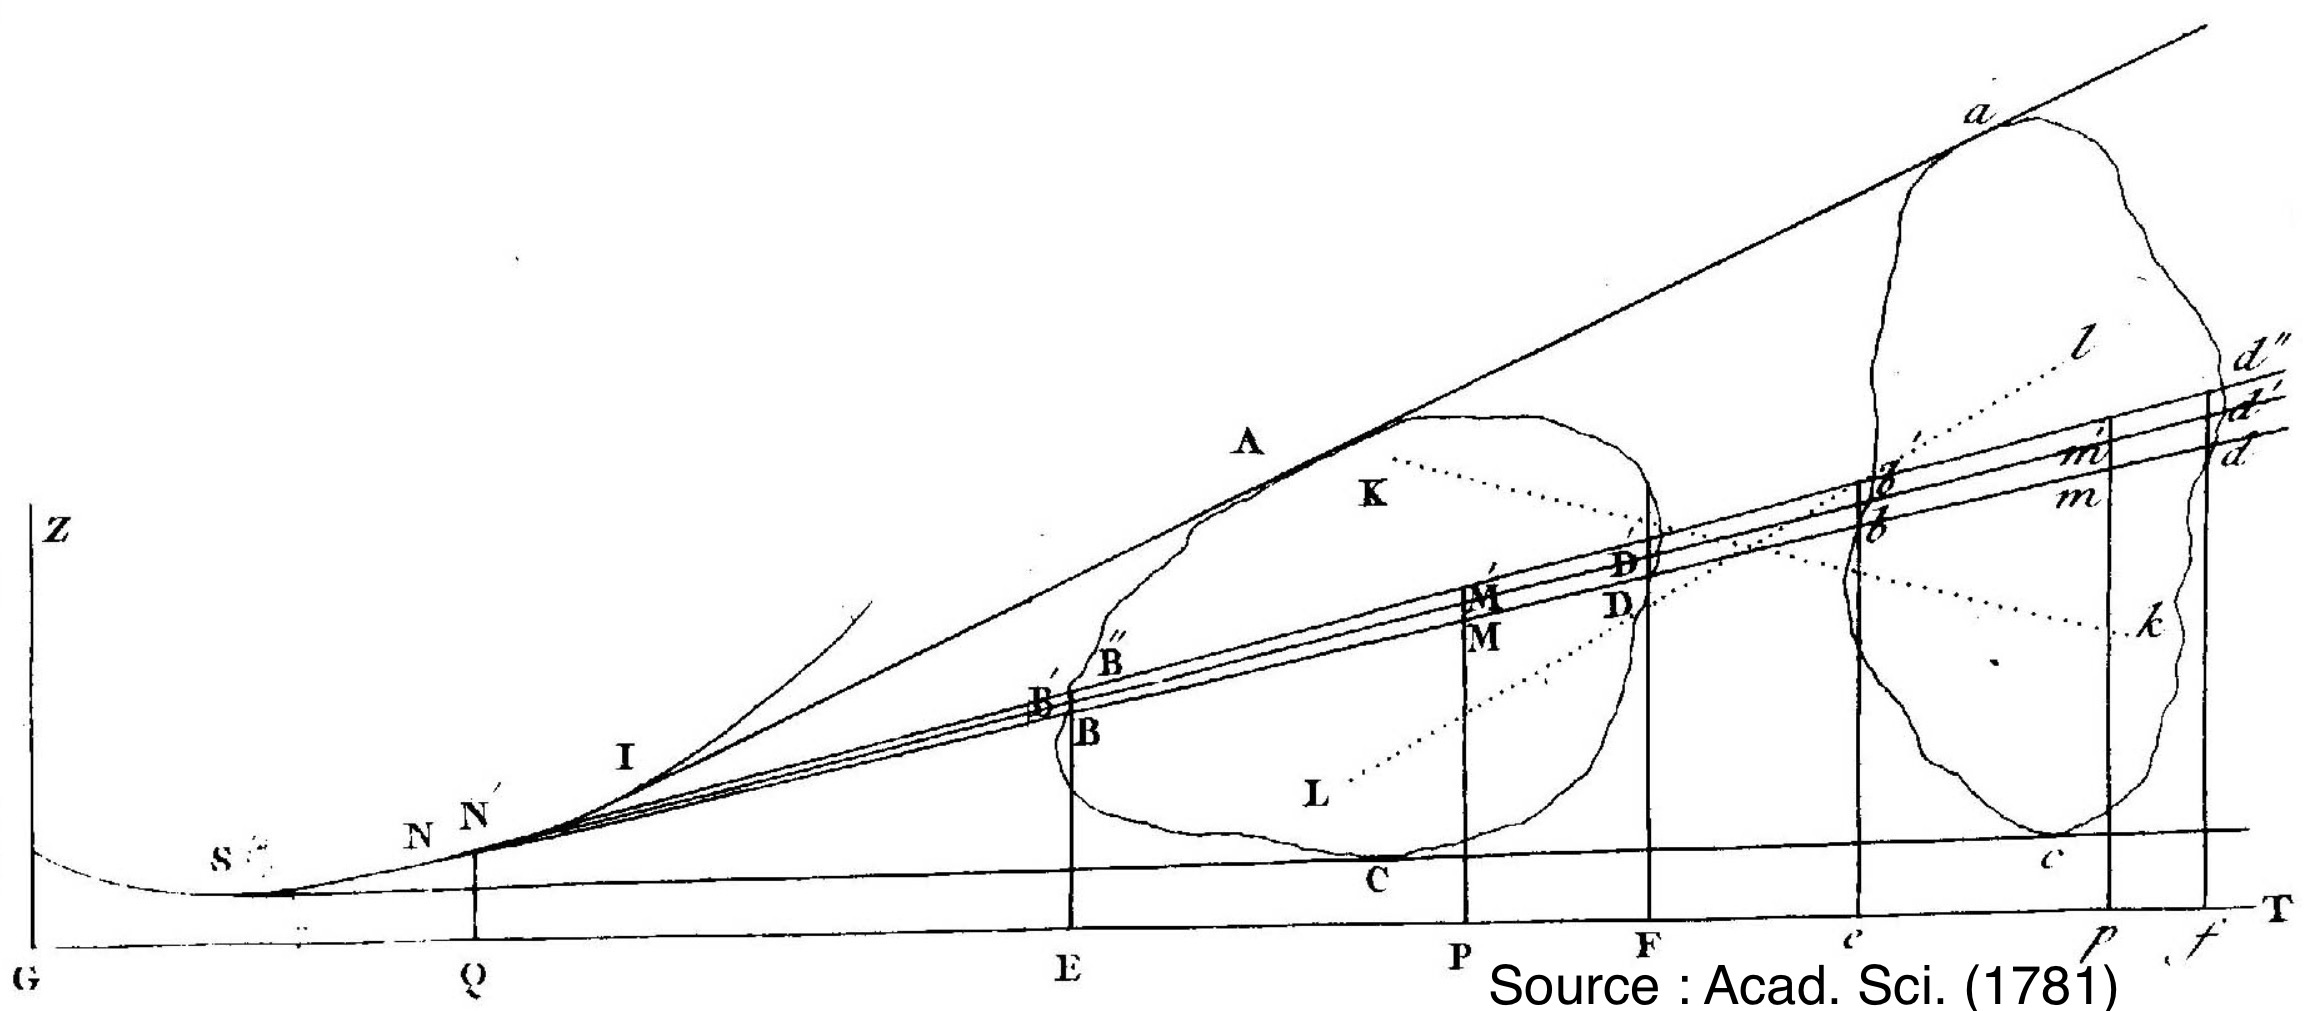
\includegraphics[height=5.0cm]{deblais}

\end{frame}

% 4. D\'eblais et remblais
\begin{frame}
\frametitle{\bf 4. D\'eblais et remblais}
 
\centering 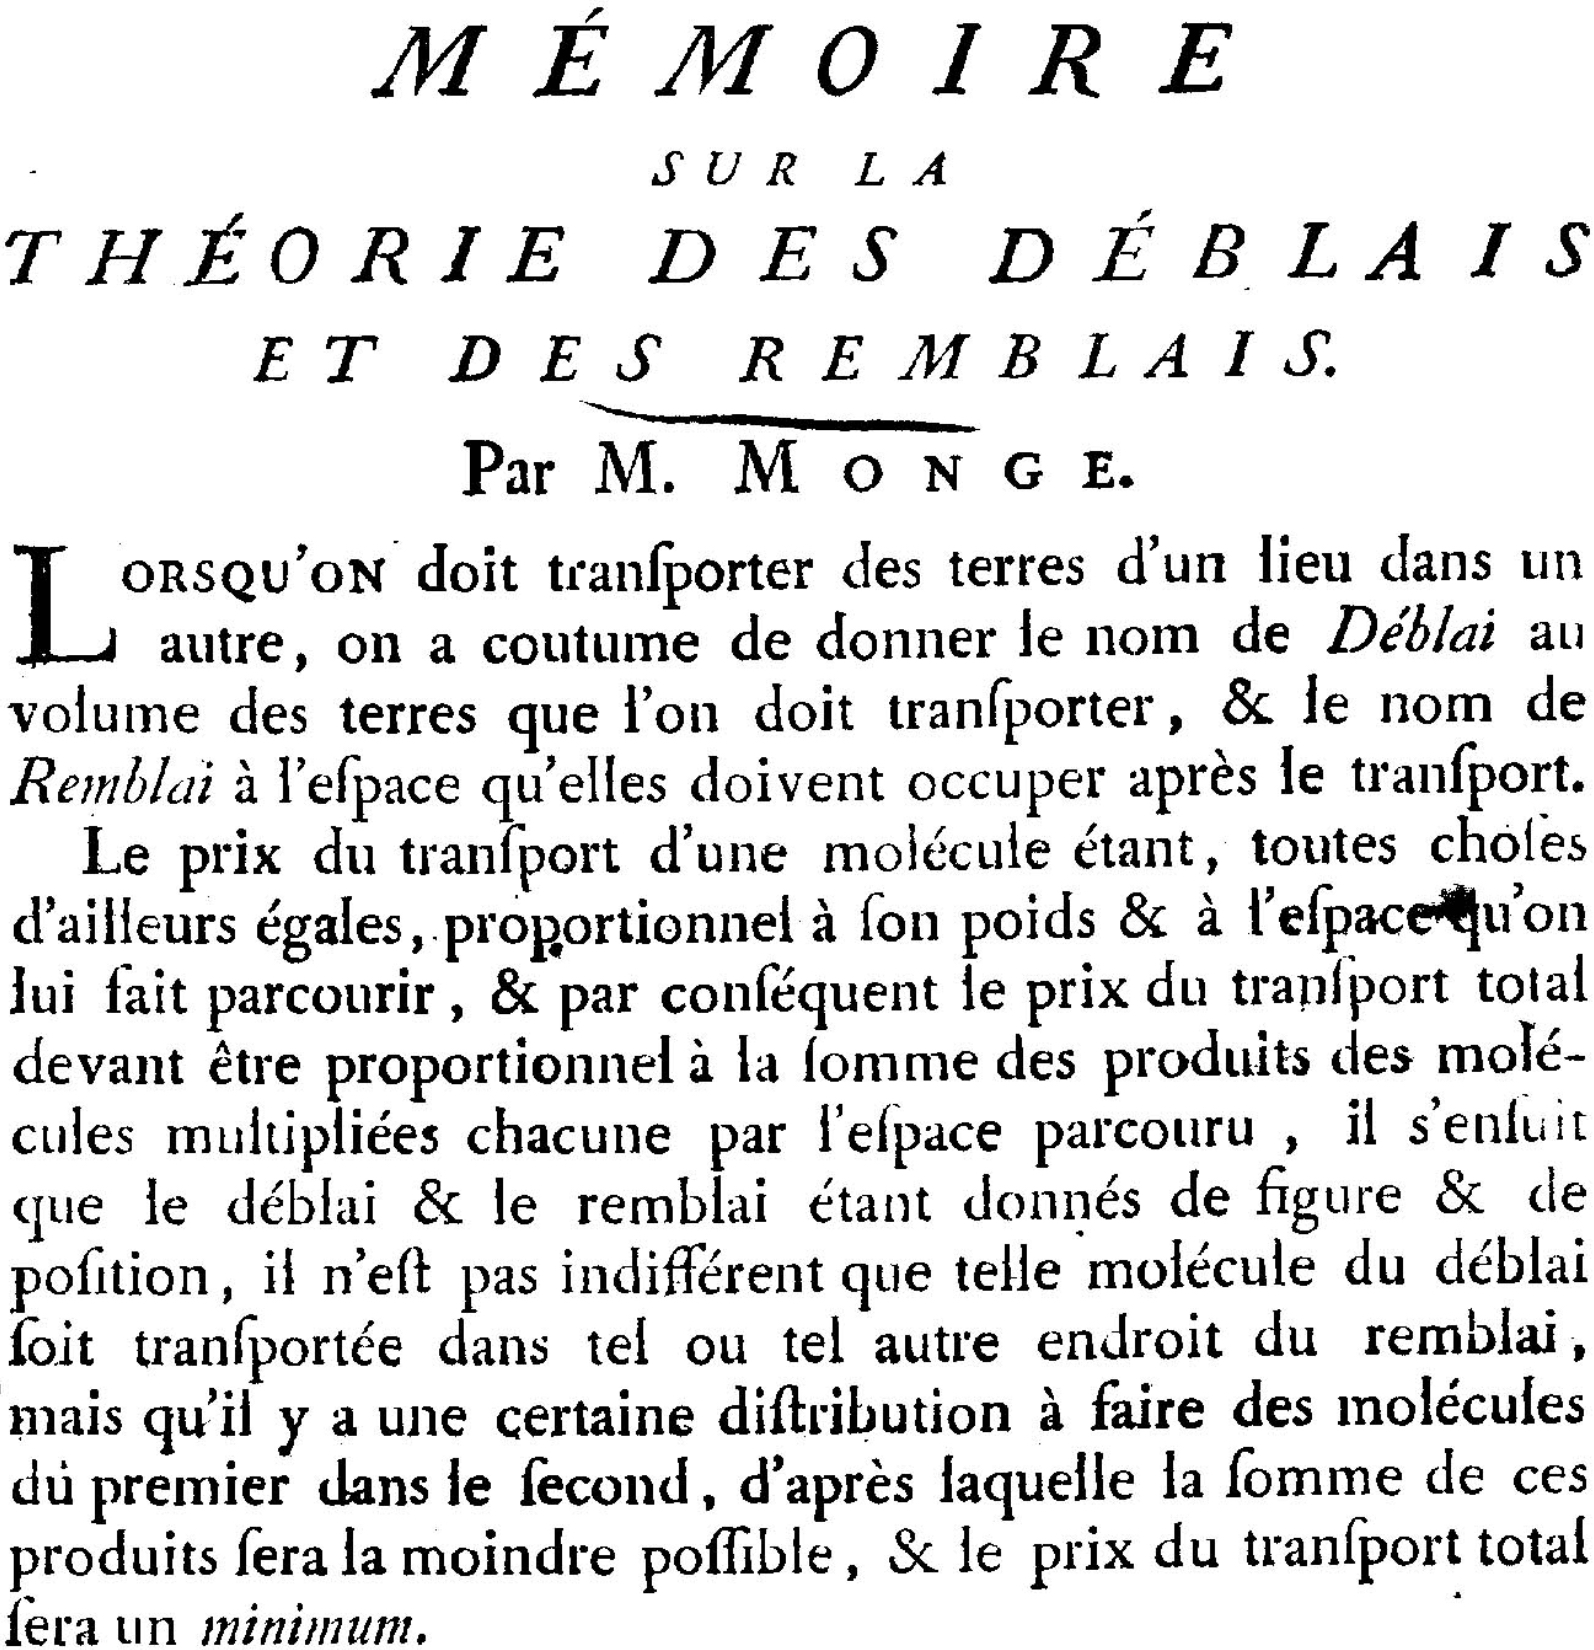
\includegraphics[height=6.0cm]{deblais2}

\end{frame}

% Transport optimal
\begin{frame}
\frametitle{\bf Transport optimal}
 
\centering 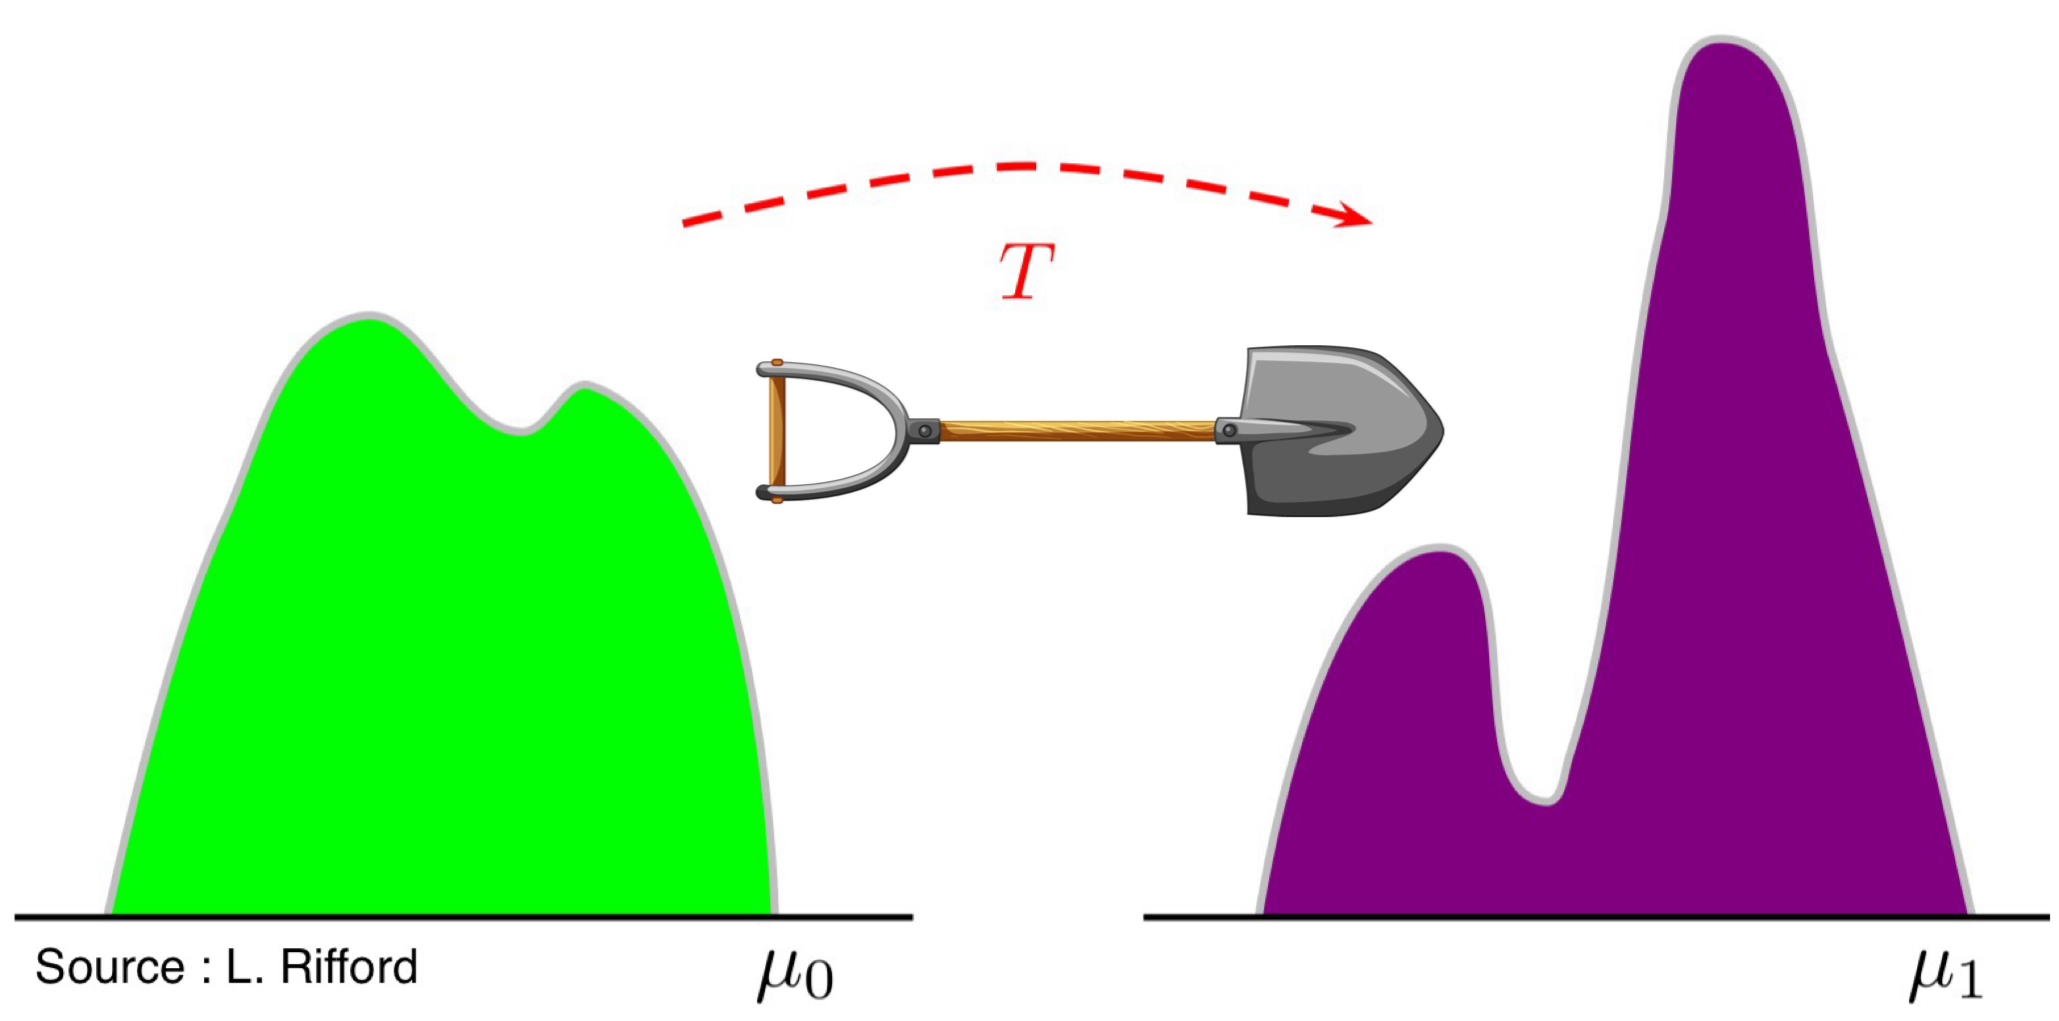
\includegraphics[height=5.0cm]{ot1}

\end{frame}

% Transport optimal
\begin{frame}
\frametitle{\bf Transport optimal}
 
\centering 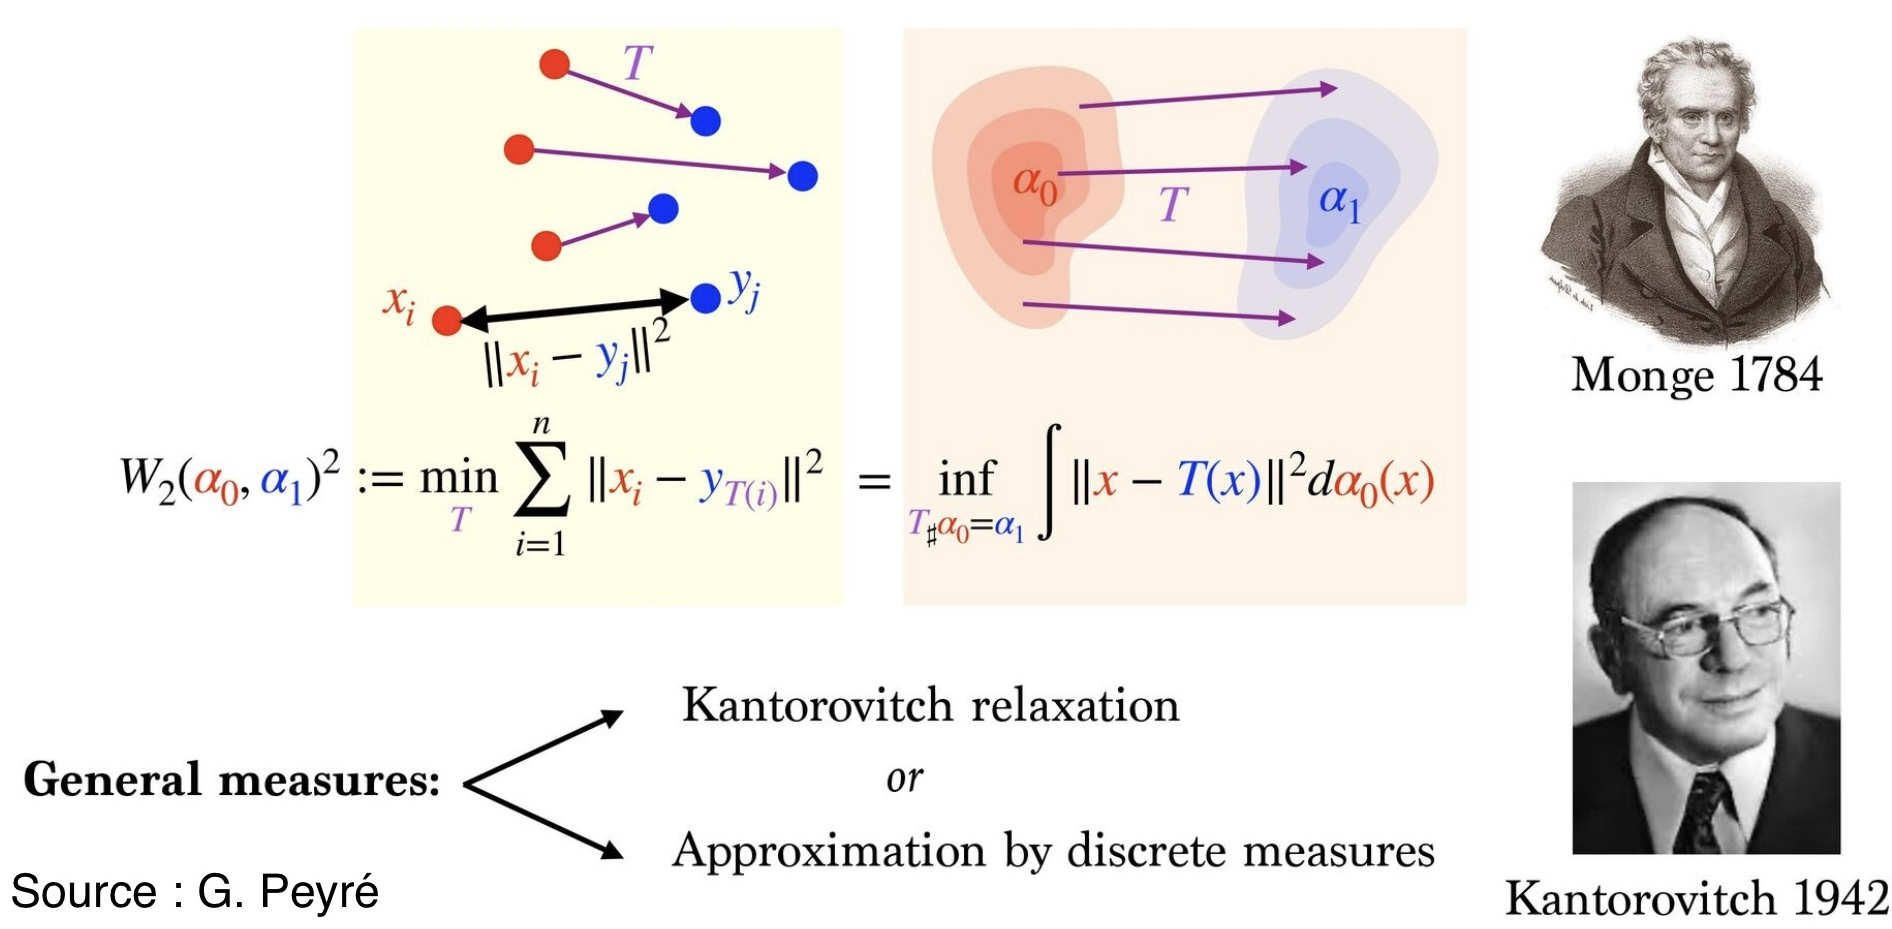
\includegraphics[height=5.5cm]{ot2}

\end{frame}

% Exemple
\begin{frame}
\frametitle{\bf Exemple}
 
\centering 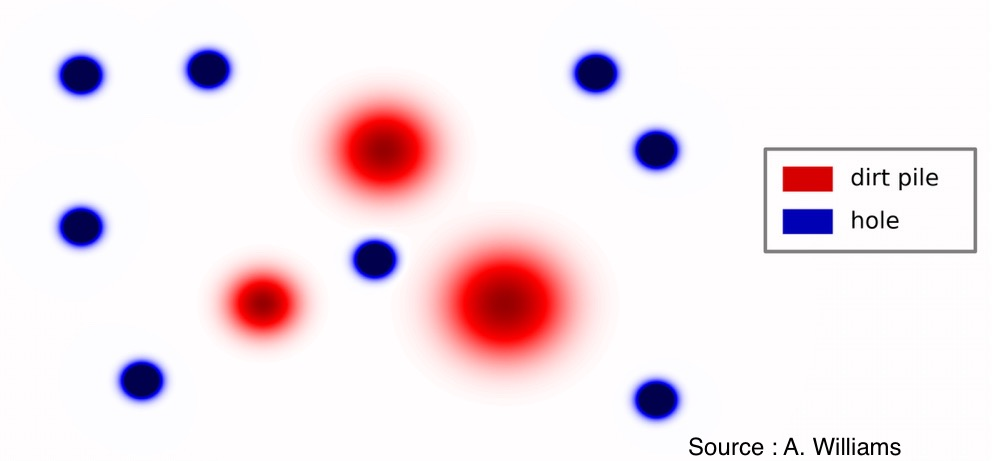
\includegraphics[height=5.0cm]{ex1}

\end{frame}

% Exemple
\begin{frame}
\frametitle{\bf Exemple}
 
\centering 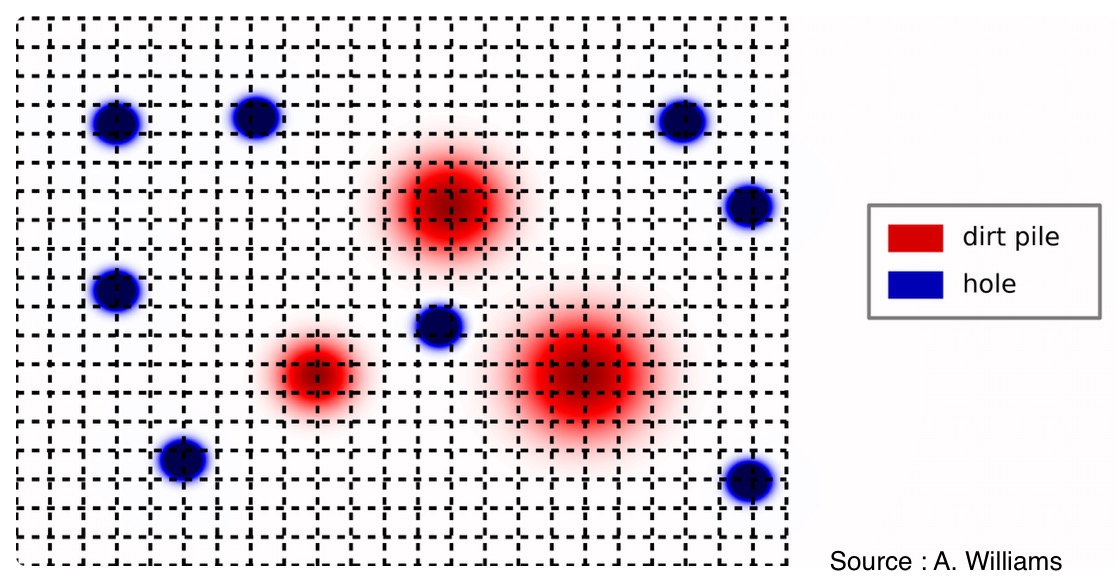
\includegraphics[height=5.0cm]{ex2}

\end{frame}

% Exemple
\begin{frame}
\frametitle{\bf Exemple}
 
\centering 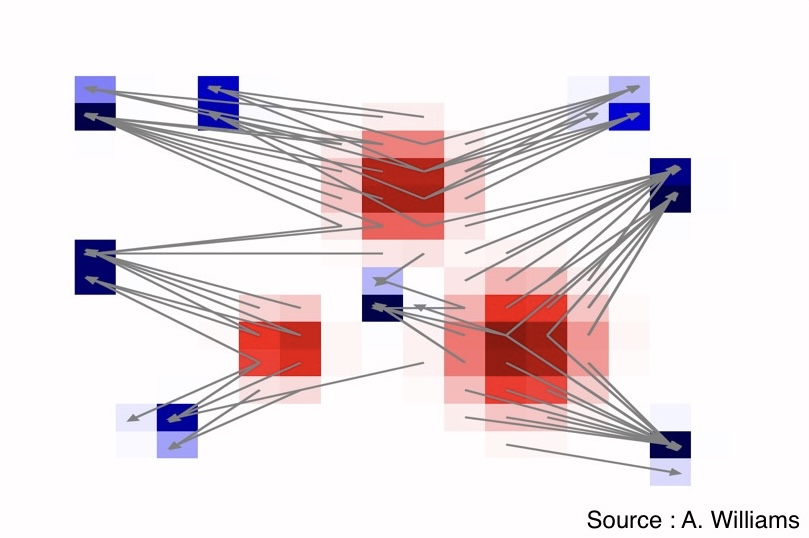
\includegraphics[height=6.0cm]{ex3}

\end{frame}

% Avec de la courbure
\begin{frame}
\frametitle{\bf Avec de la courbure}
 
\centering 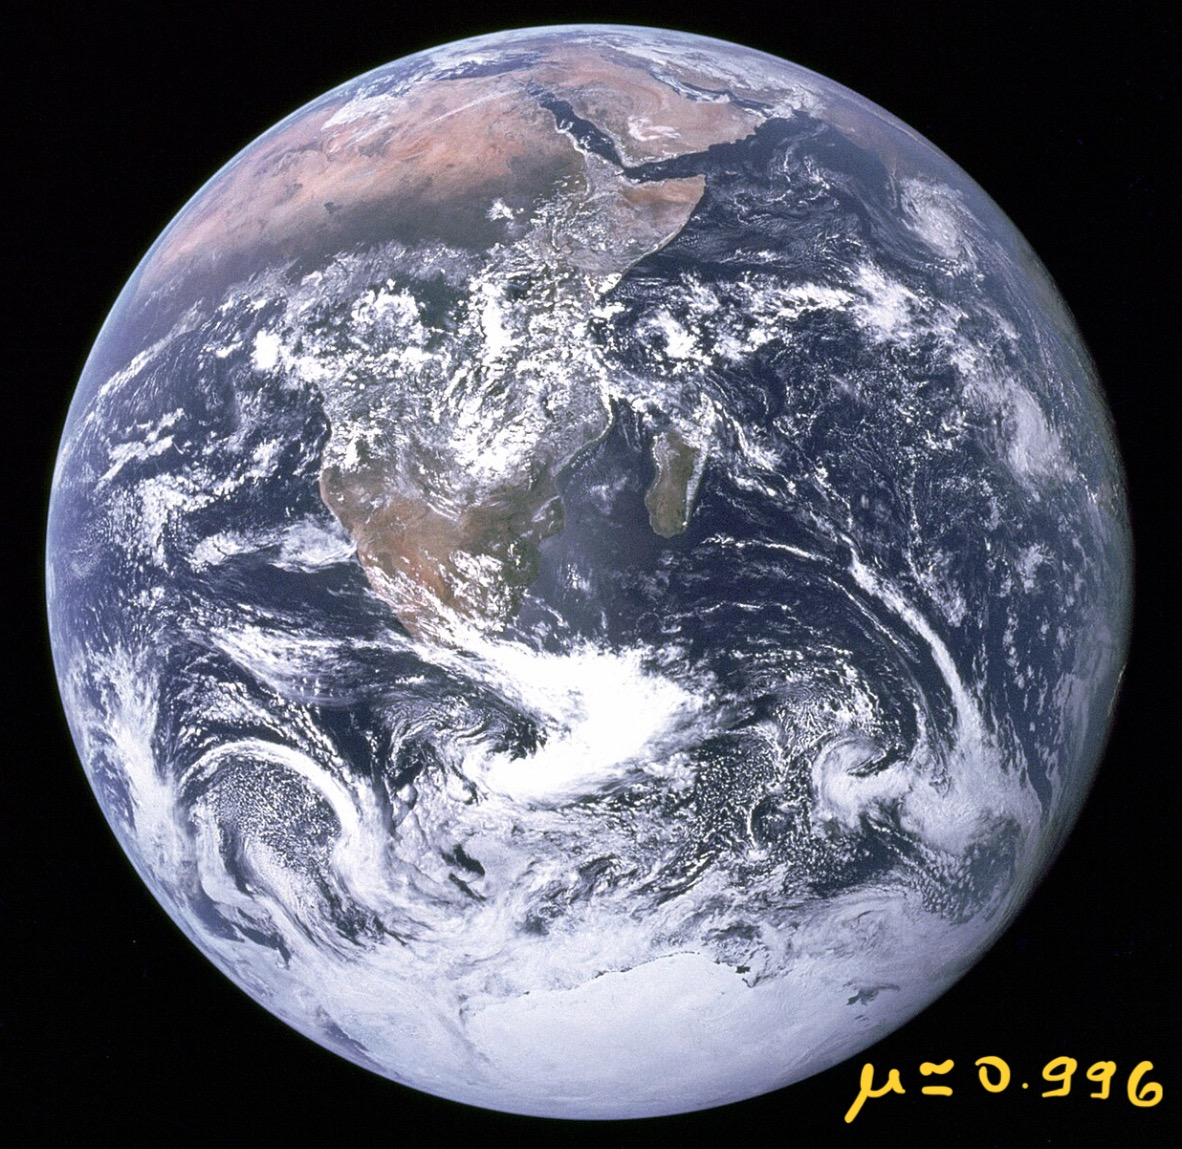
\includegraphics[height=7.0cm]{terre}

\end{frame}

% Avec plus de courbure
\begin{frame}
\frametitle{\bf Avec plus de courbure}
 
\centering 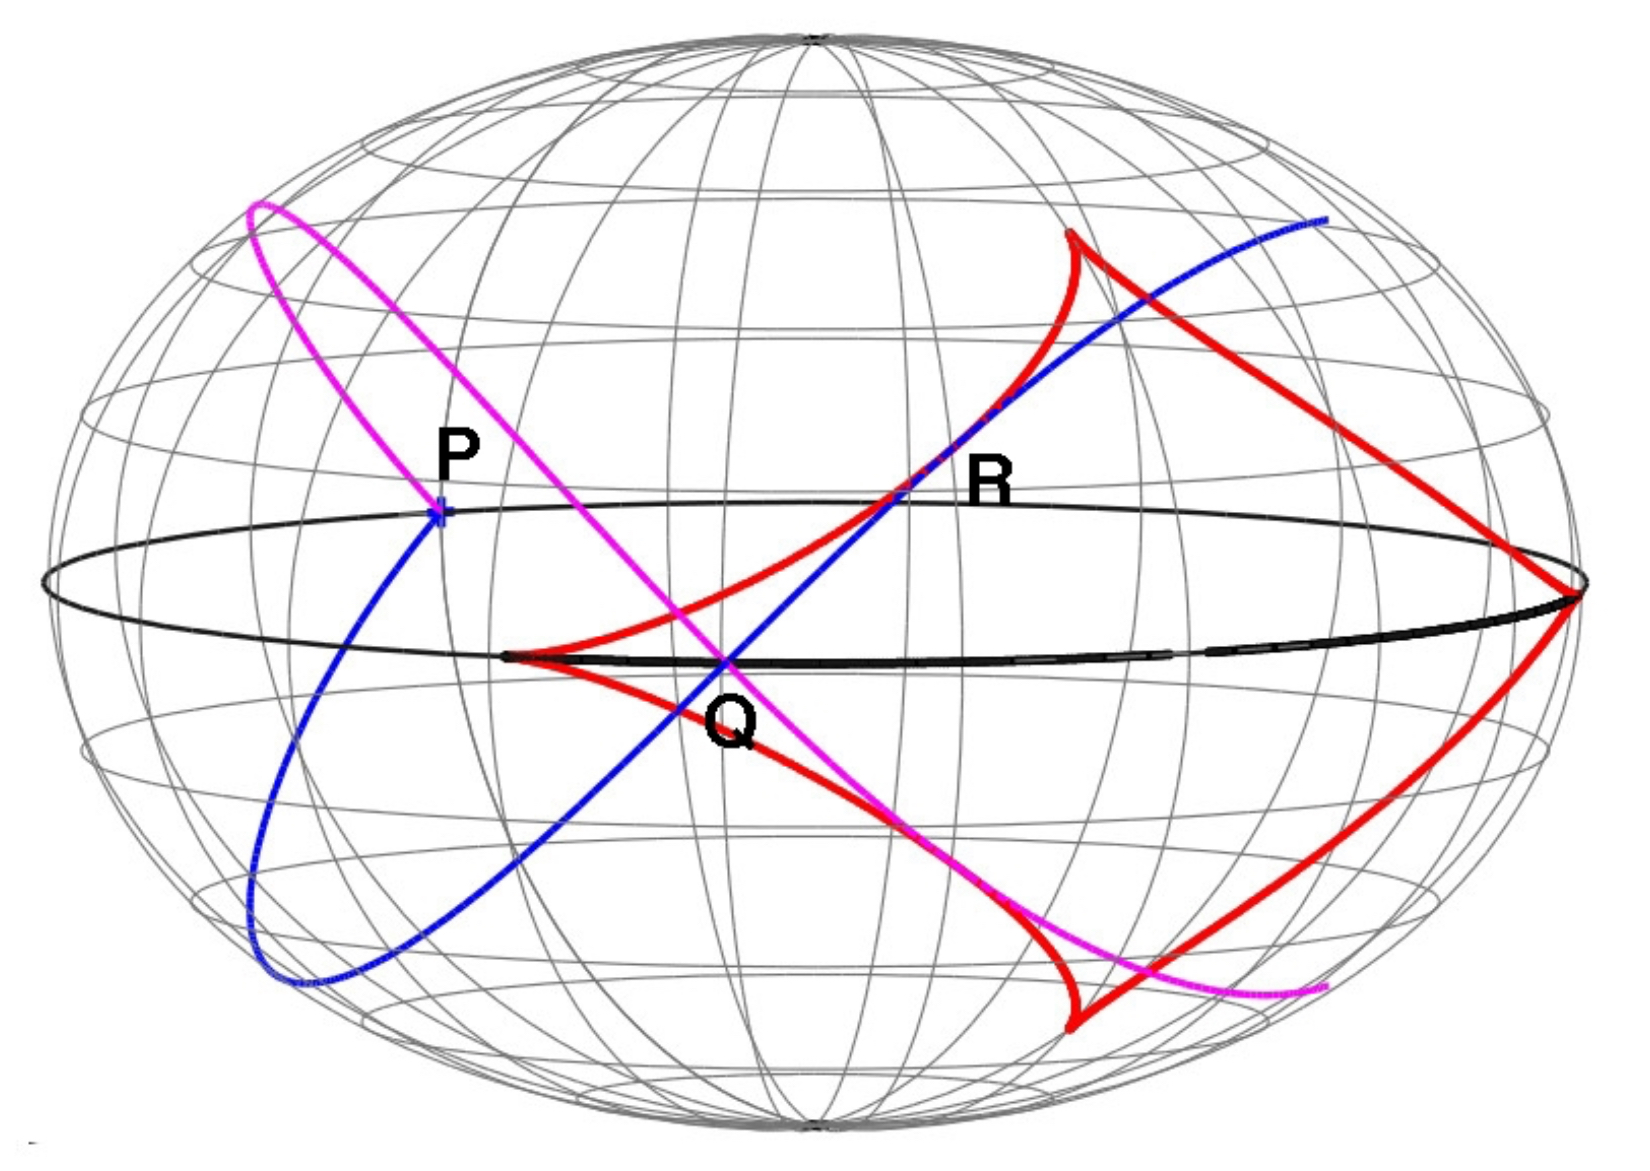
\includegraphics[height=5.0cm]{ellip}

\begin{itemize}
  \item Existence ?
  \item Unicit\'e ?
  \item R\'egularit\'e ?
\end{itemize}

\end{frame}

% Obstruction \`a la continuit\'e
\begin{frame}
\frametitle{\bf Obstruction \`a la continuit\'e}
 
\centering 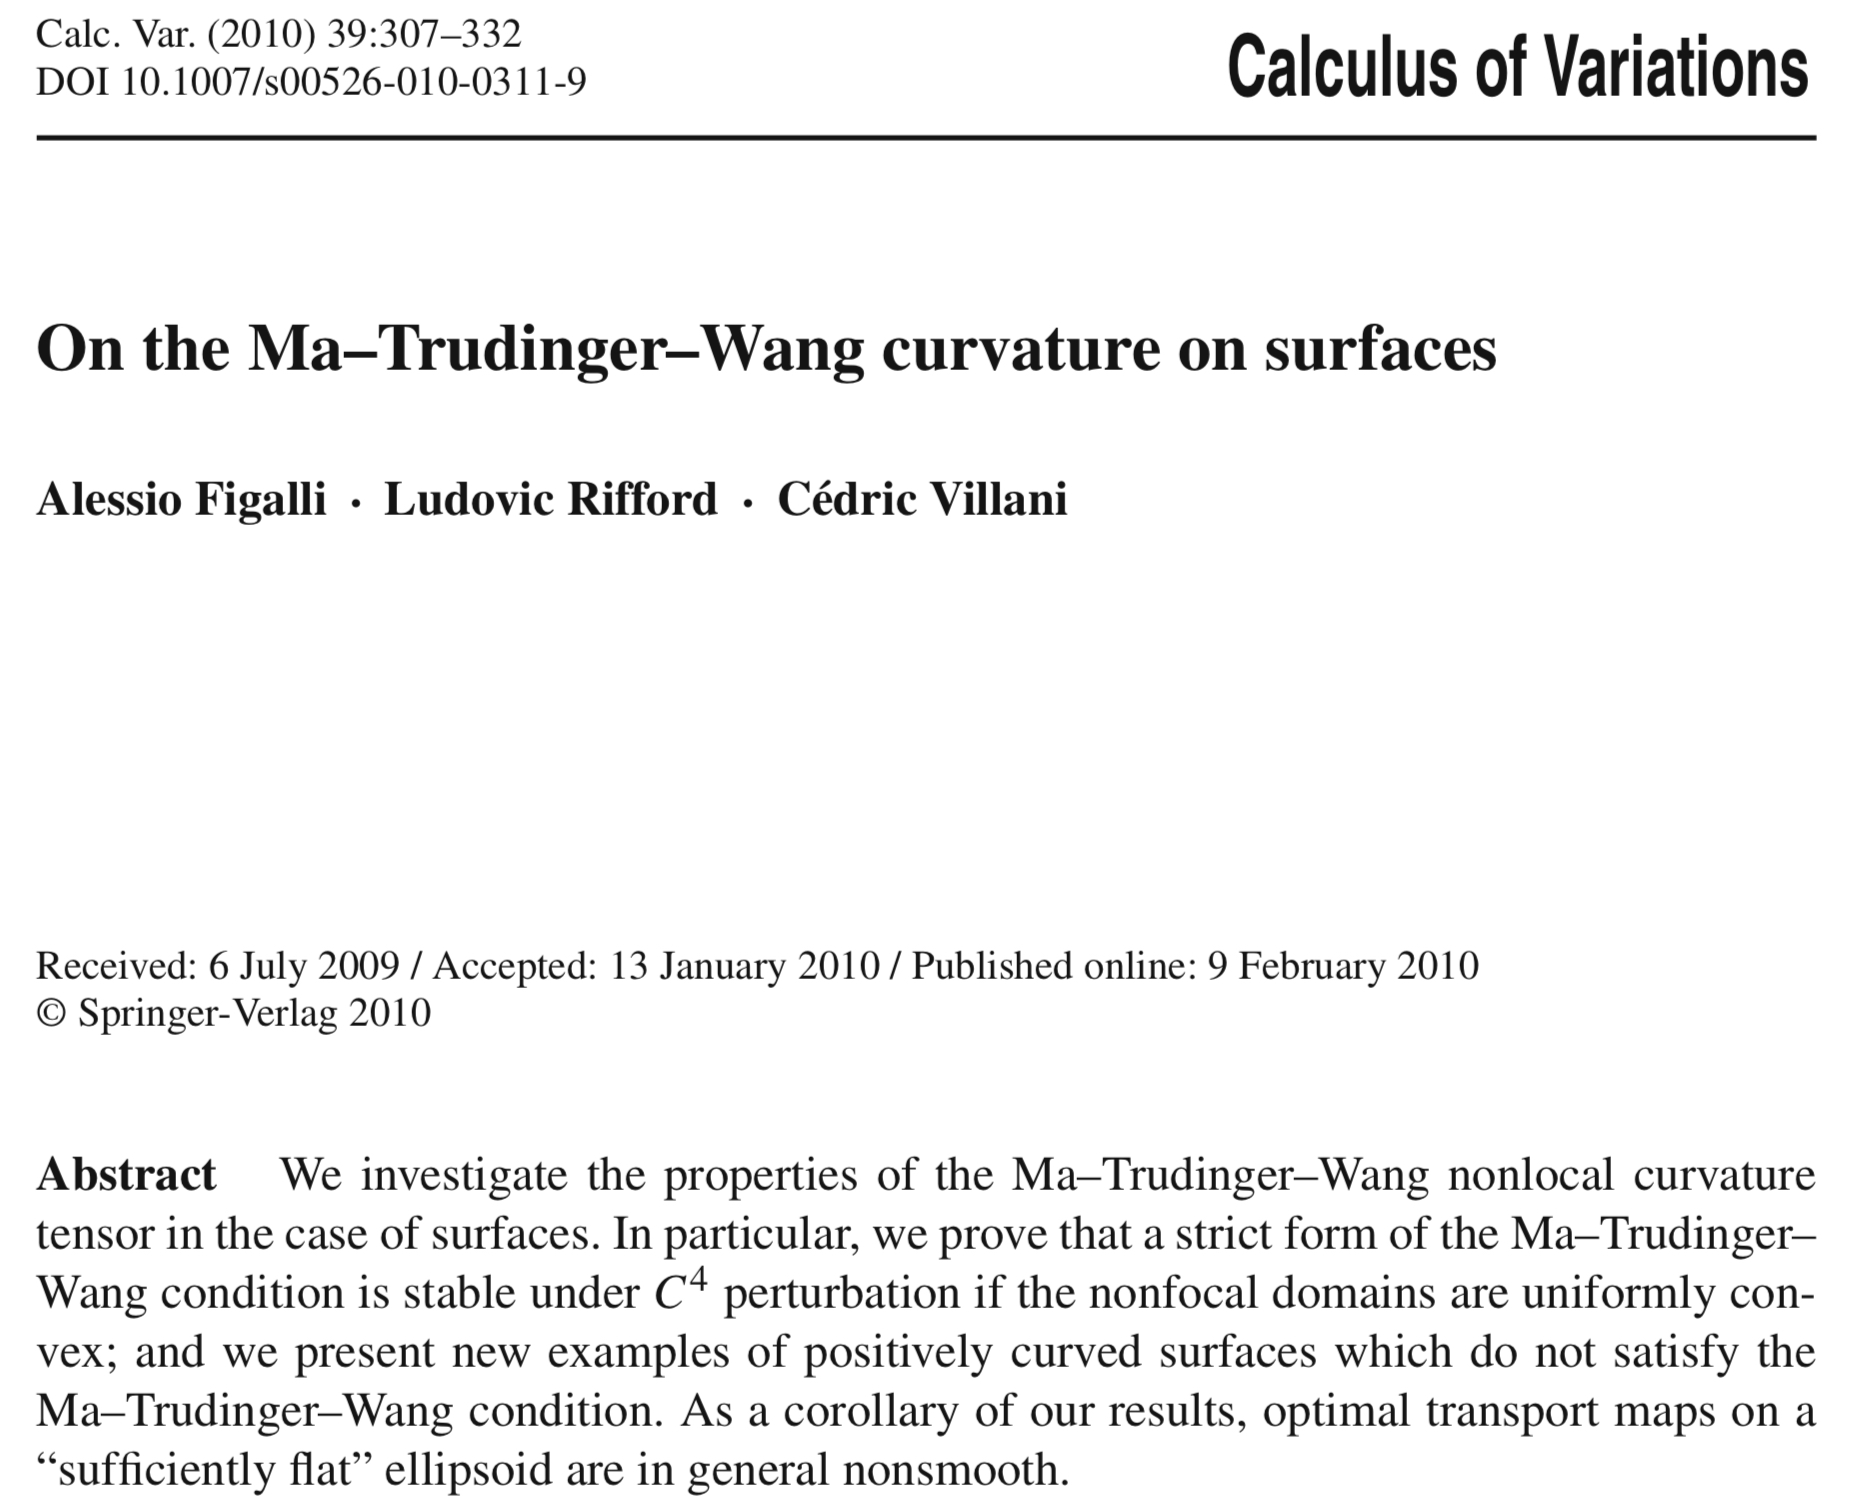
\includegraphics[height=7.0cm]{figal1}

\end{frame}

% Obstruction \`a la continuit\'e
\begin{frame}
\frametitle{\bf Obstruction \`a la continuit\'e}
 
\centering 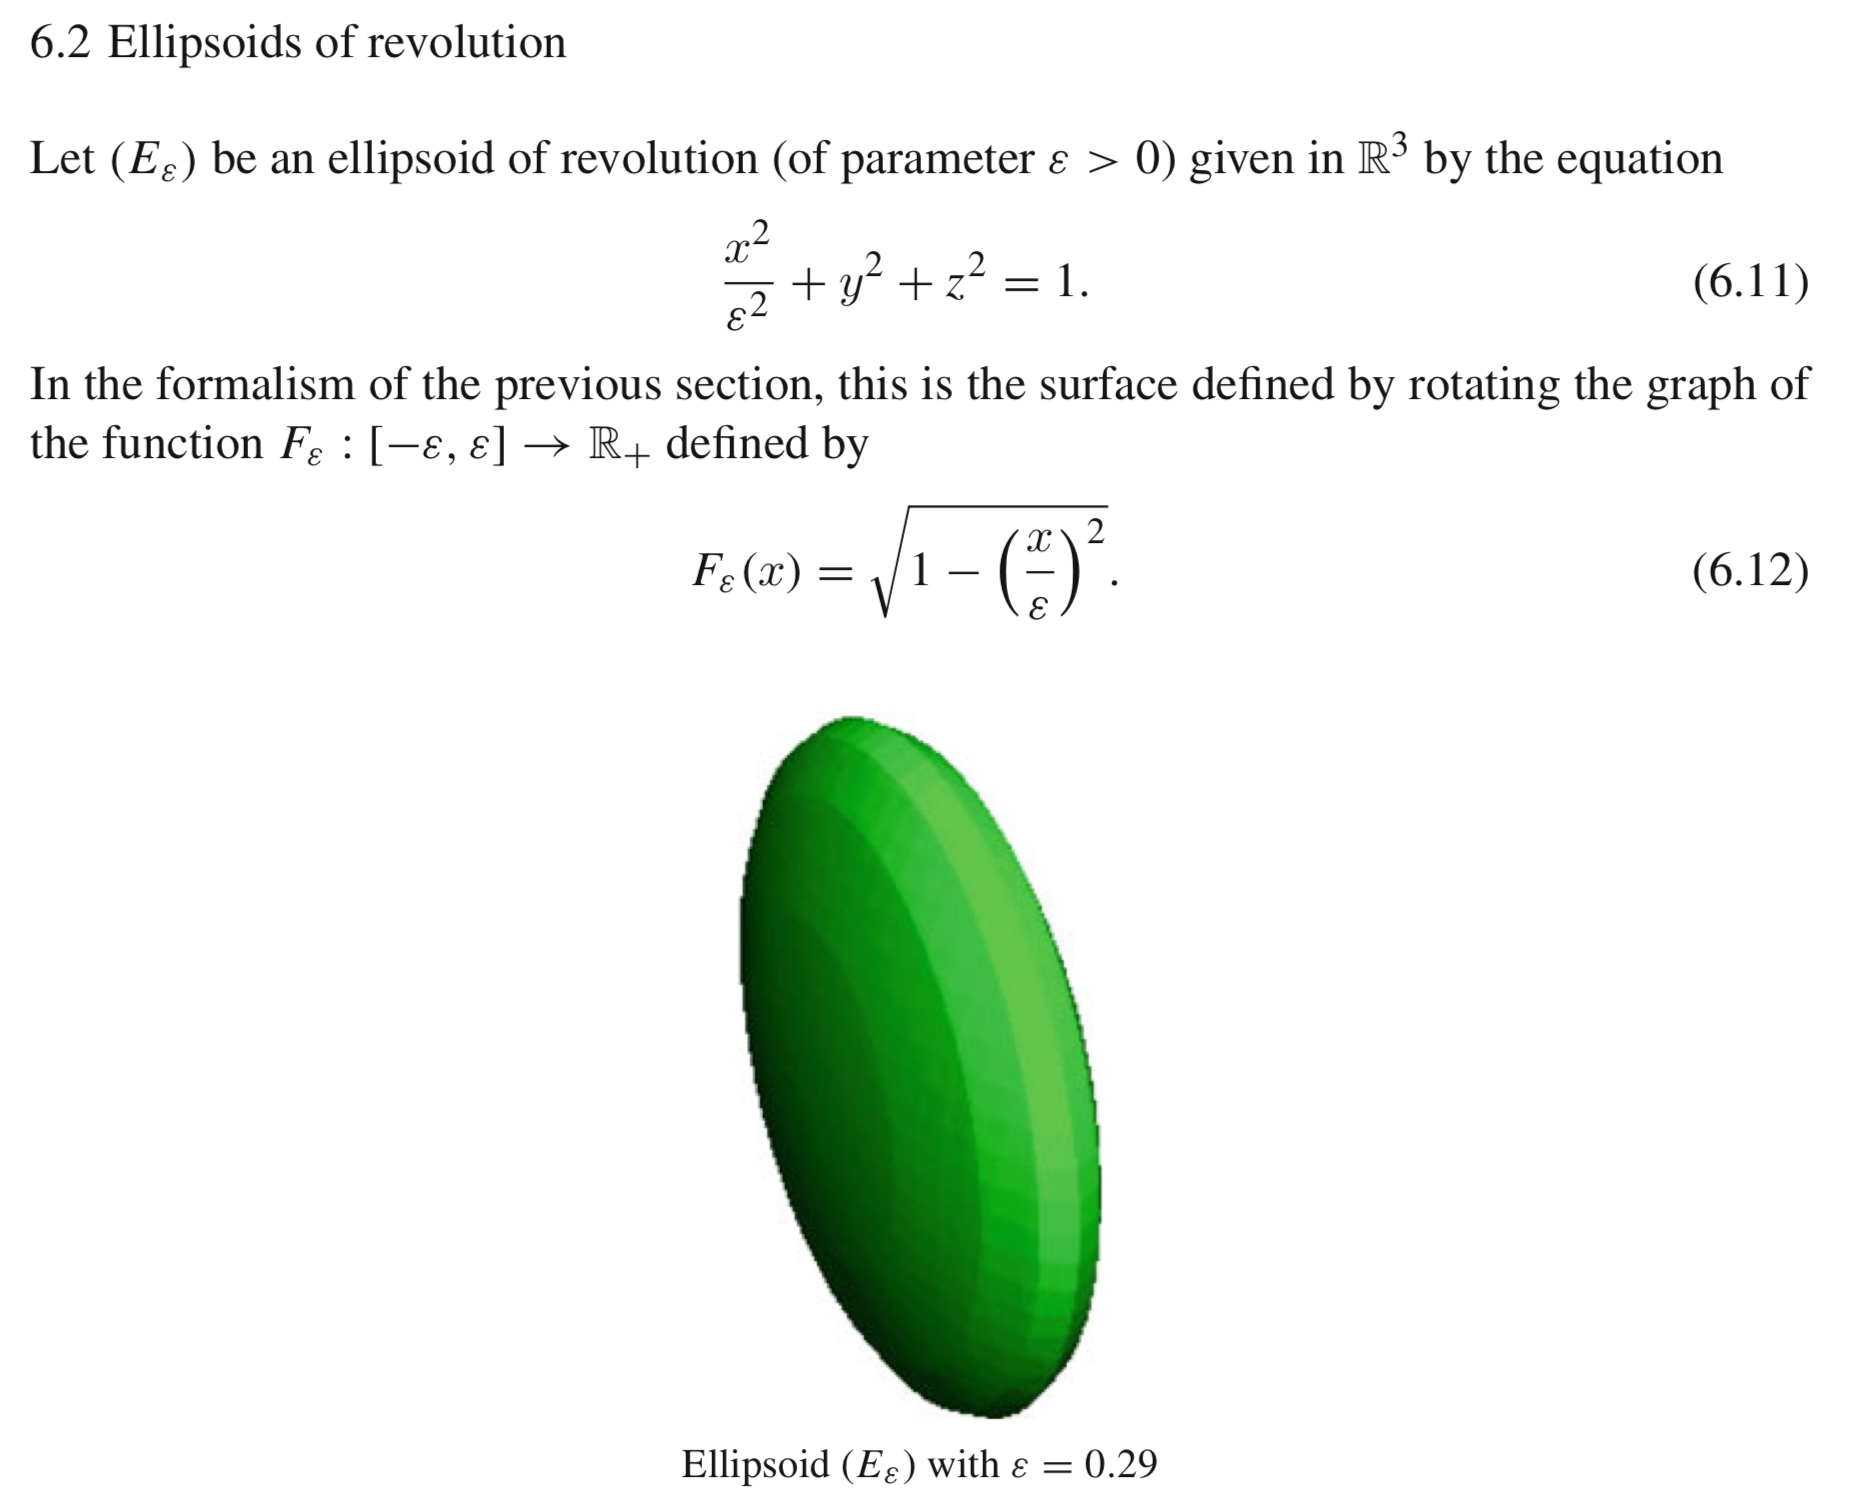
\includegraphics[height=7.0cm]{figal2}

\end{frame}

% De la terre (presque) ronde \`a la terre plate
\begin{frame}
\frametitle{\bf De la terre (presque) ronde \`a la terre plate}
 
\centering 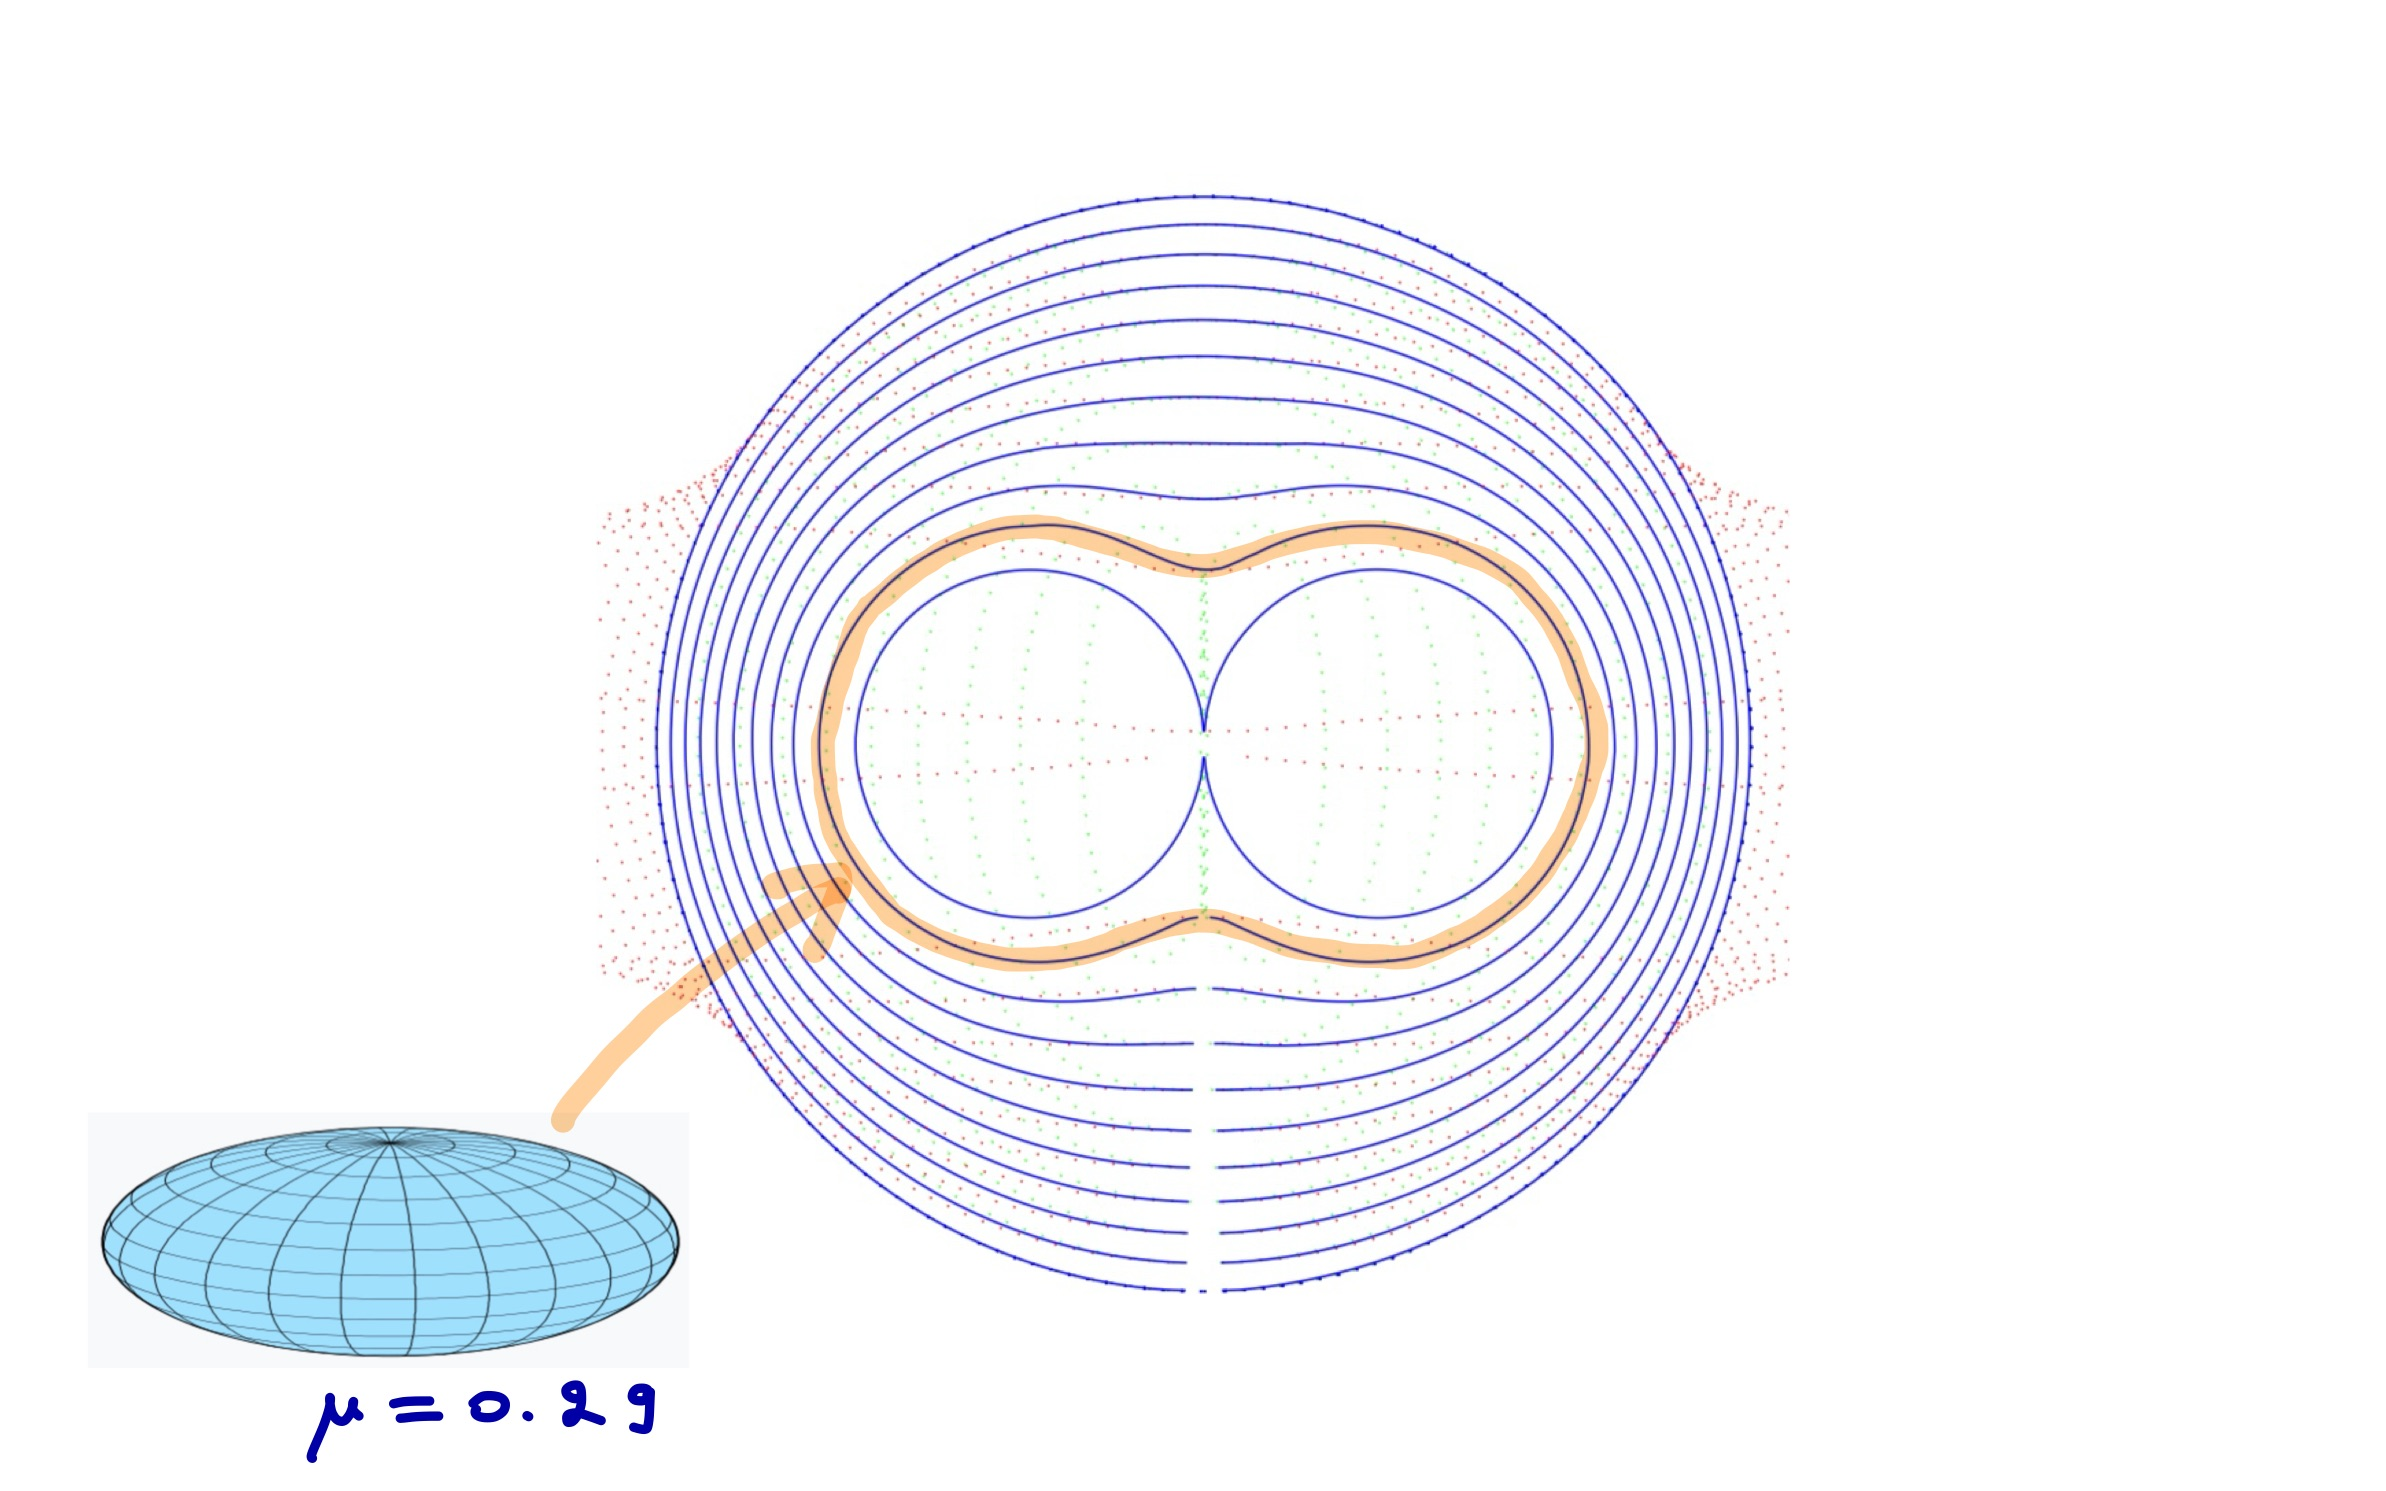
\includegraphics[height=7.0cm]{oblat1}

\end{frame}

% De la terre (presque) ronde \`a la terre plate
\begin{frame}
\frametitle{\bf De la terre (presque) ronde \`a la terre plate}
 
\centering 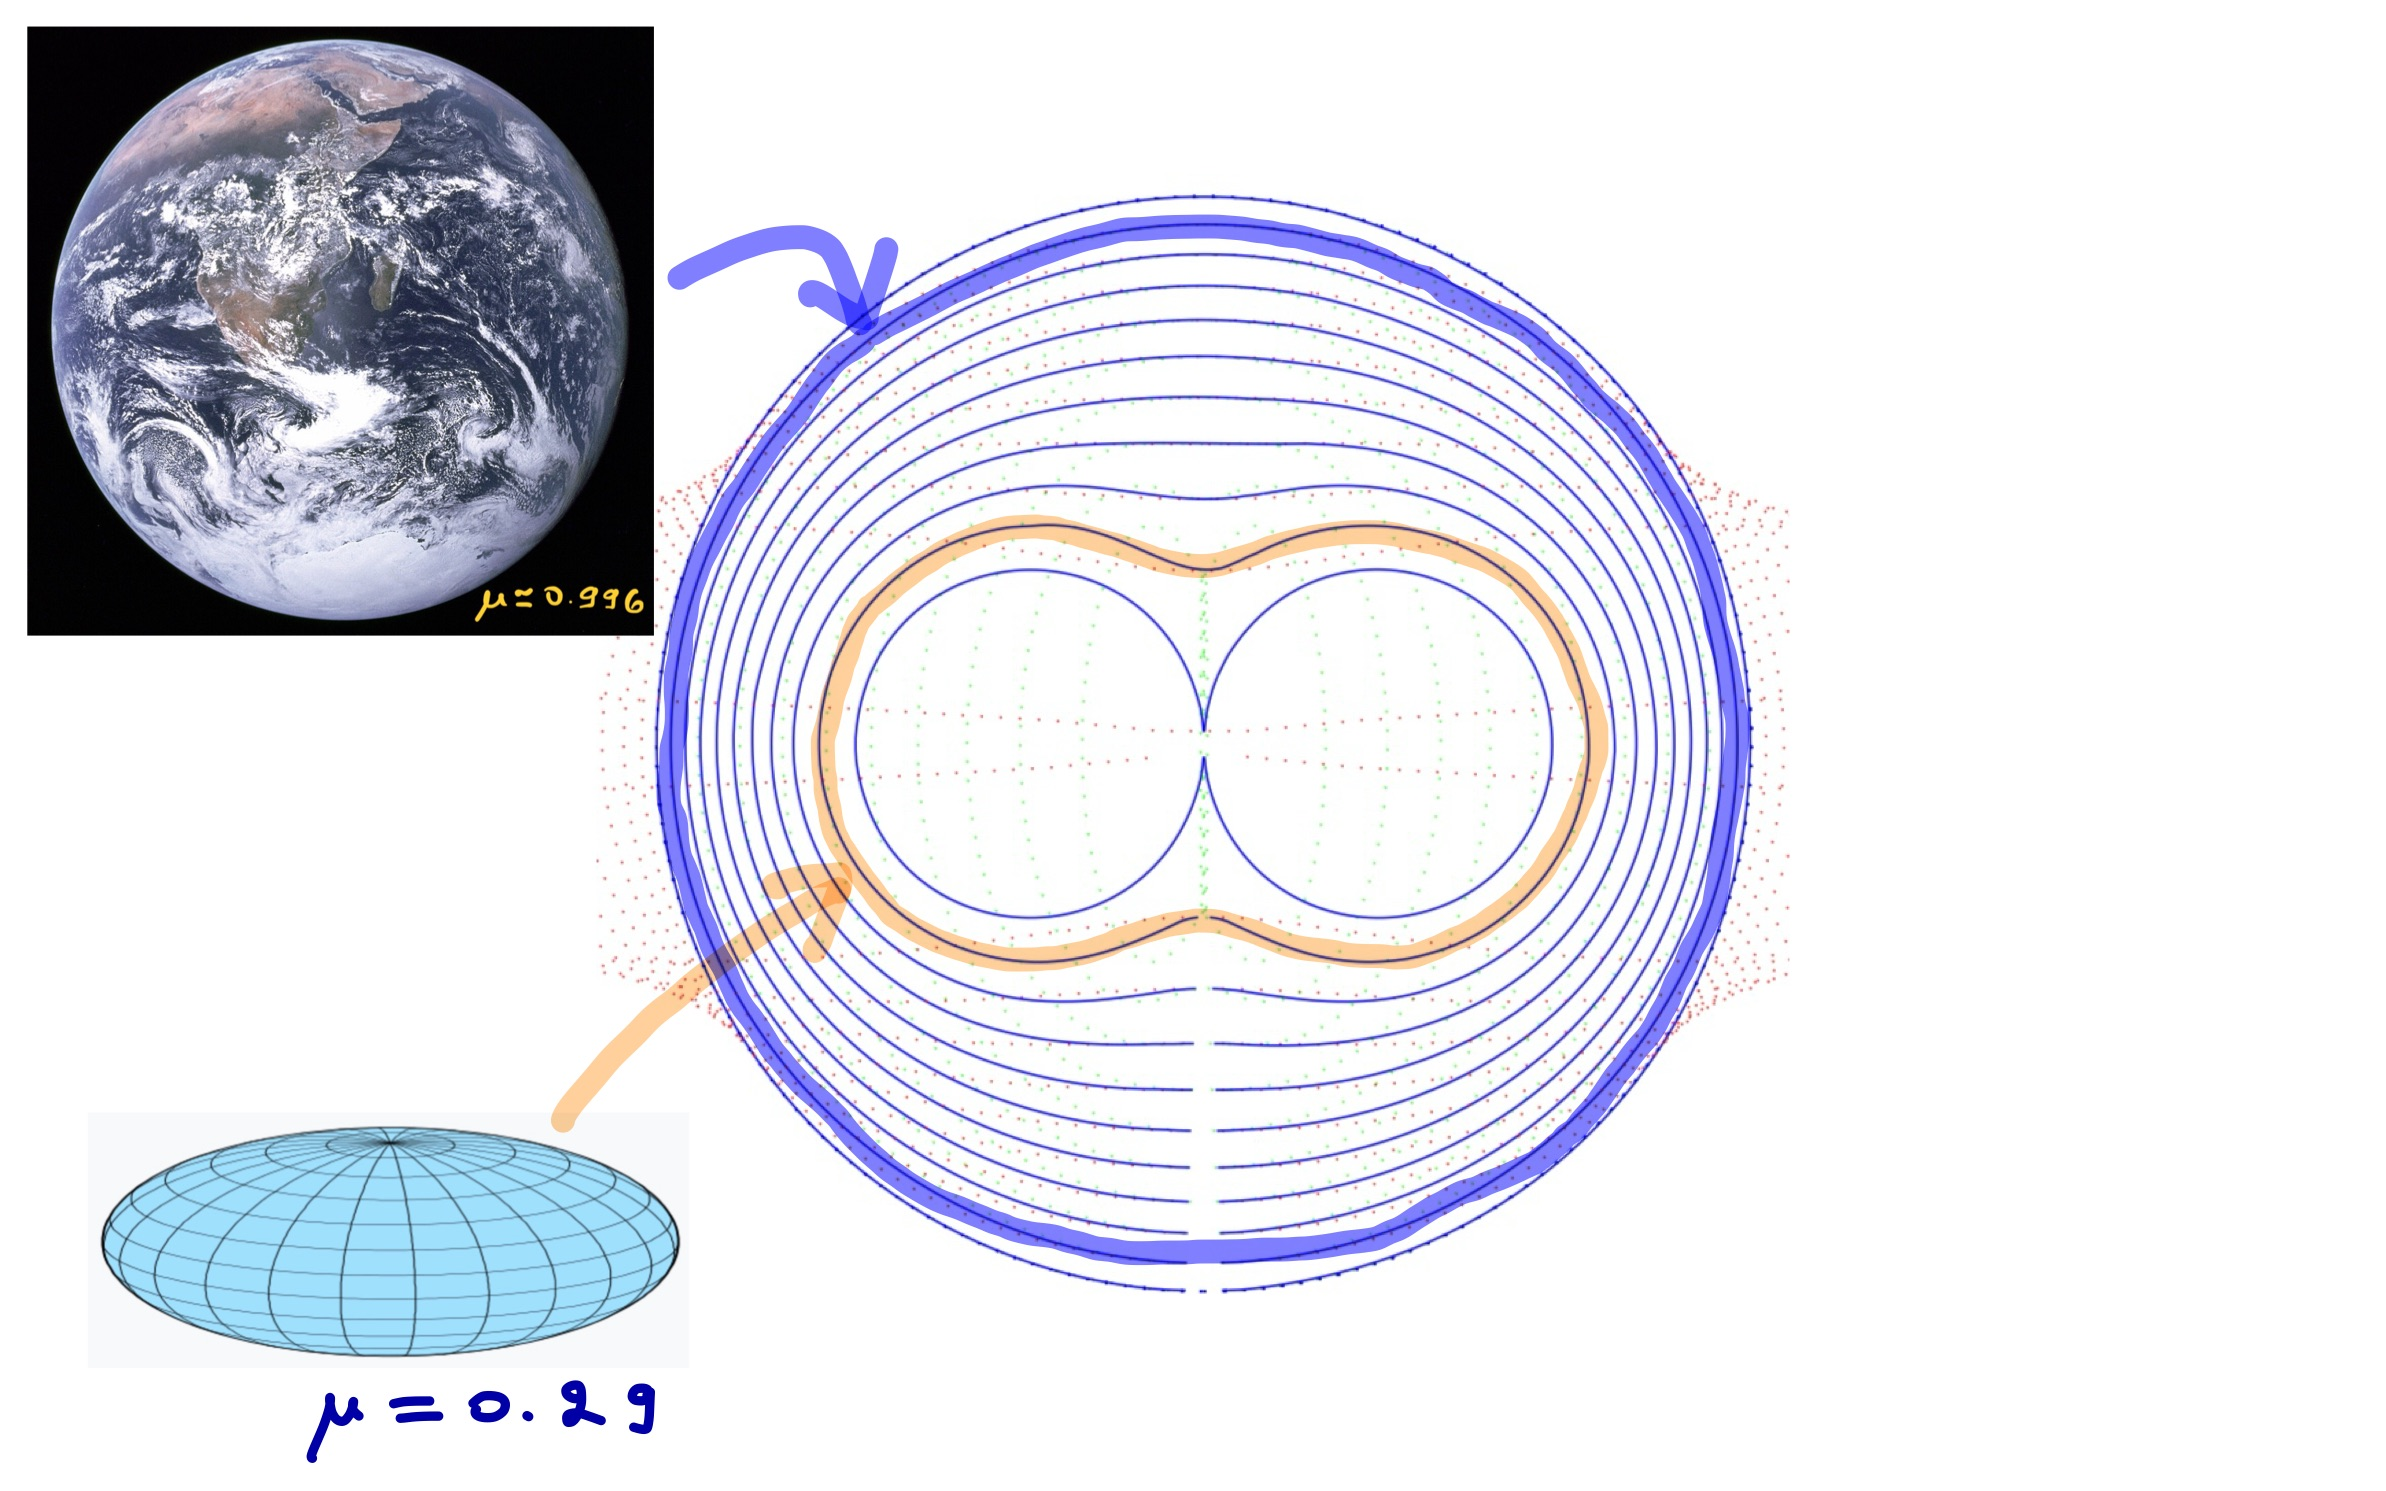
\includegraphics[height=7.0cm]{oblat2}

\end{frame}

% De la terre (presque) ronde \`a la terre plate
\begin{frame}
\frametitle{\bf De la terre (presque) ronde \`a la terre plate}
 
\centering 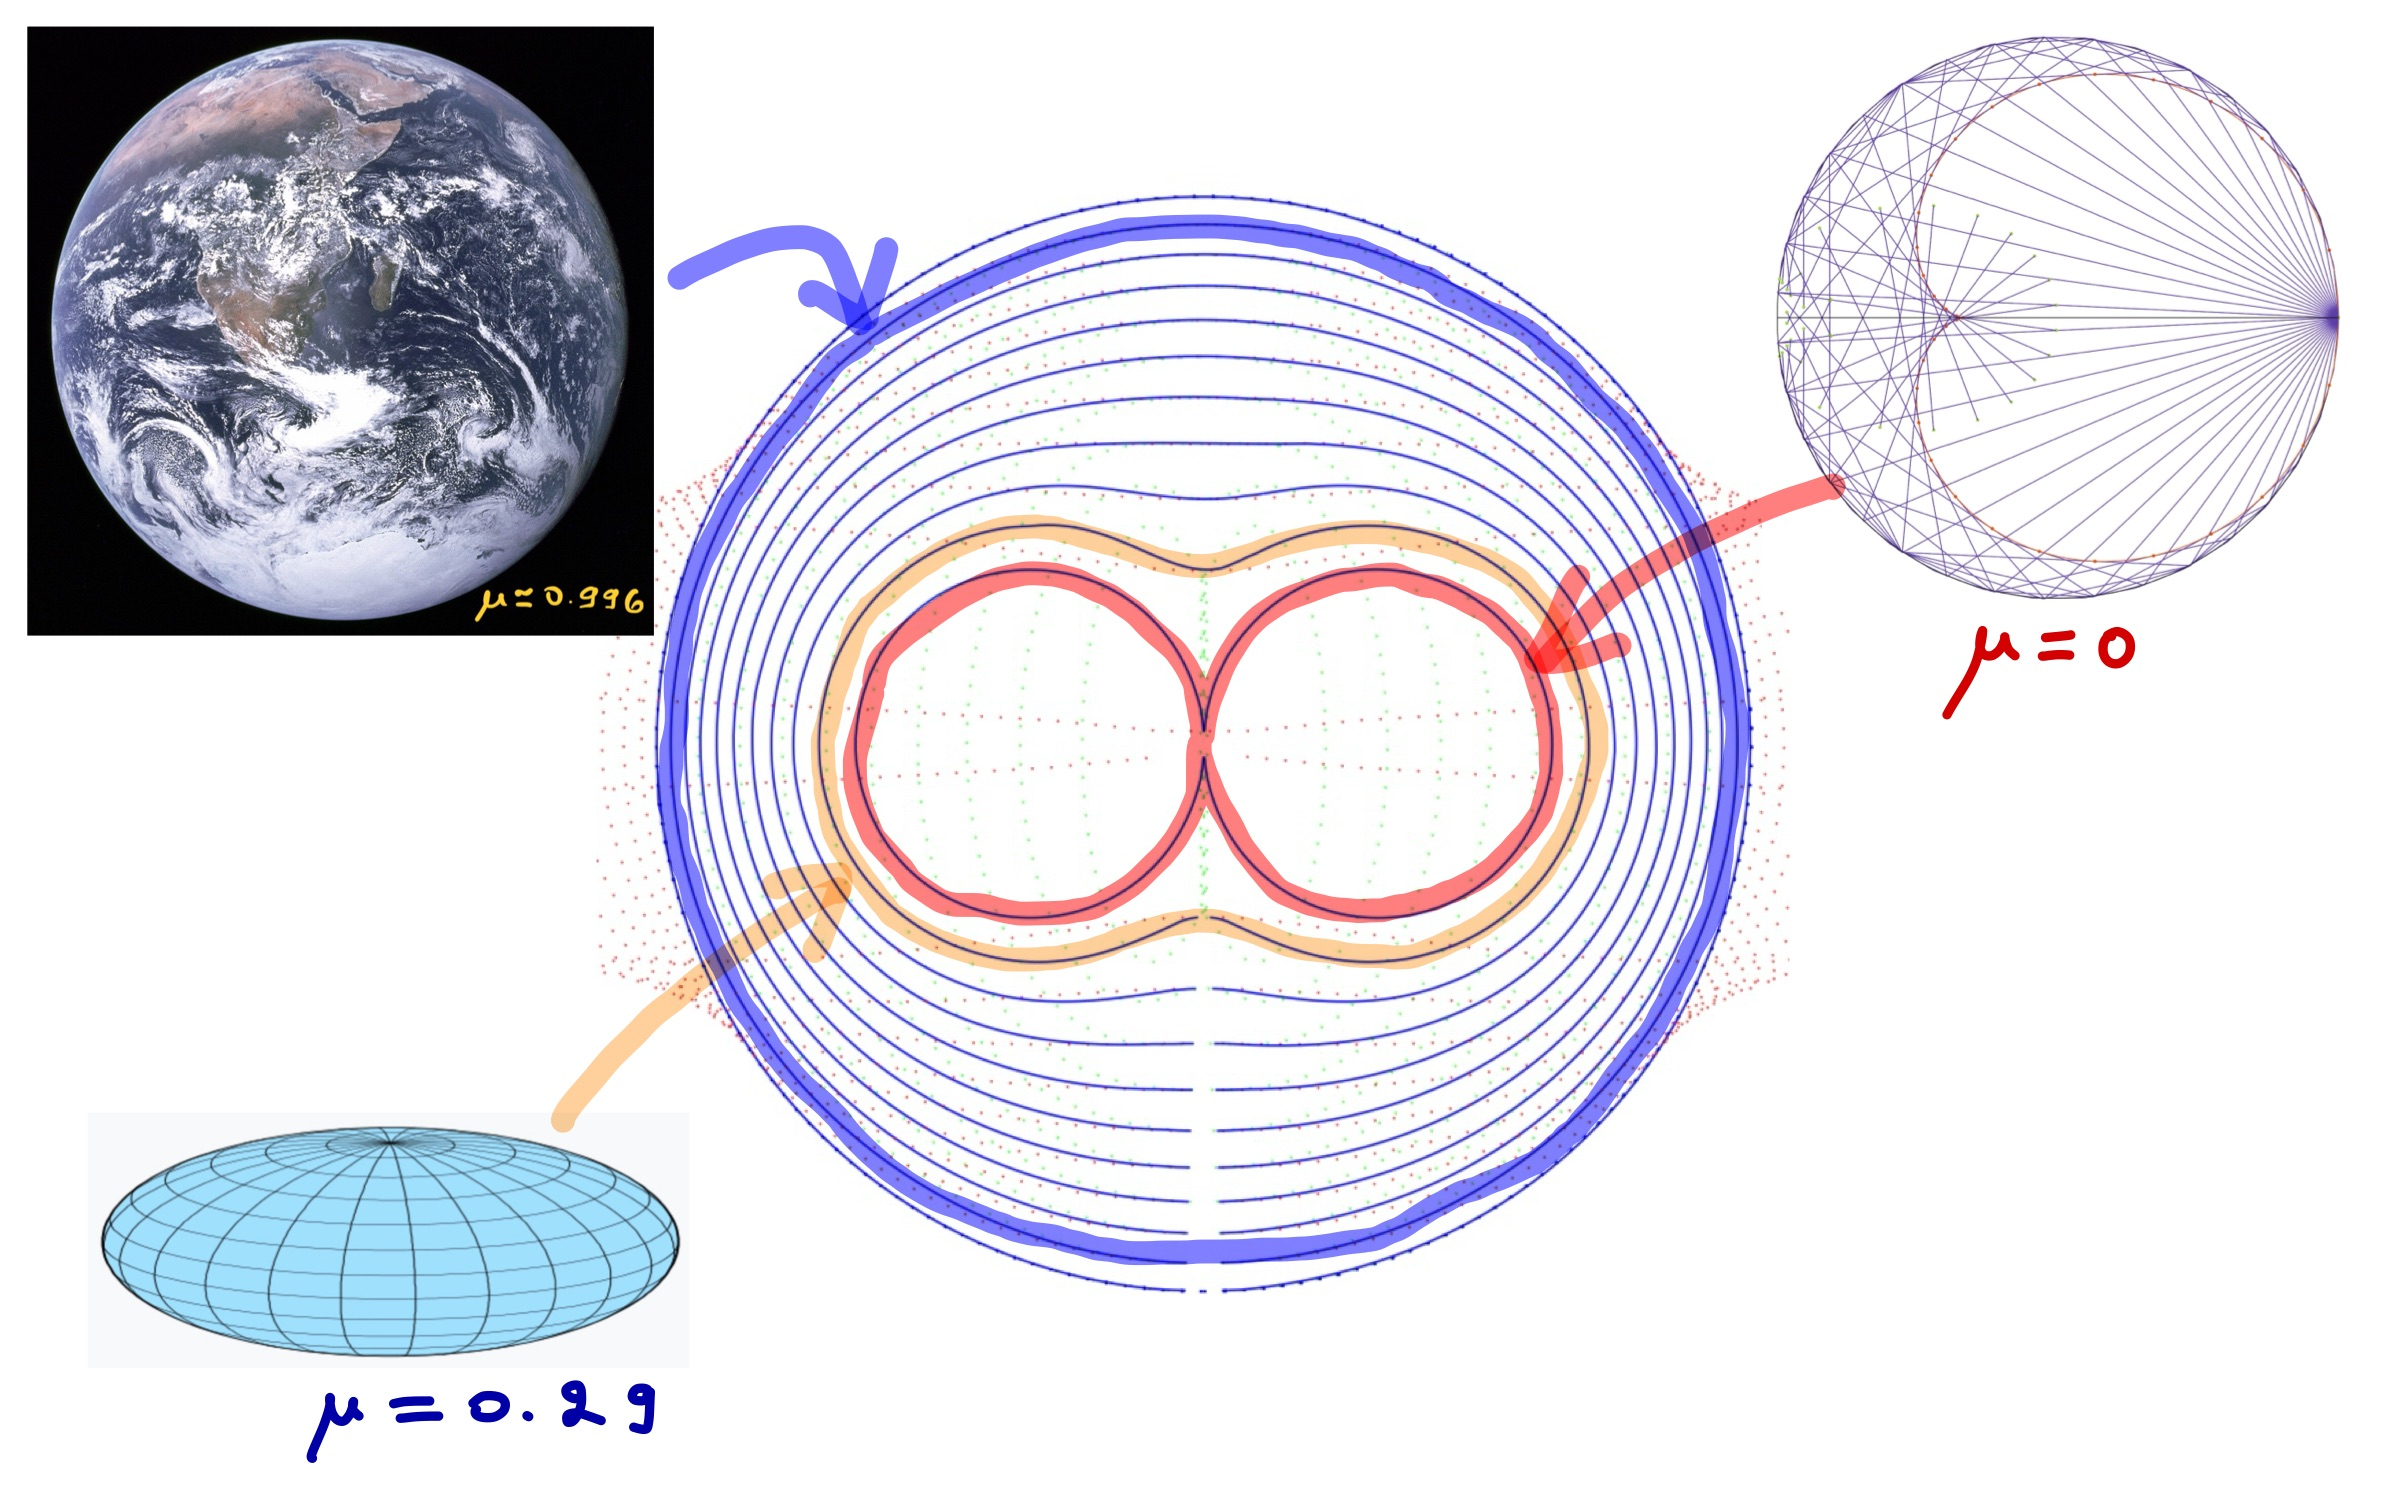
\includegraphics[height=7.0cm]{oblat3}

\end{frame}

% De la terre (presque) ronde \`a la terre plate
\begin{frame}
\frametitle{\bf De la terre (presque) ronde \`a la terre plate}
 
\centering 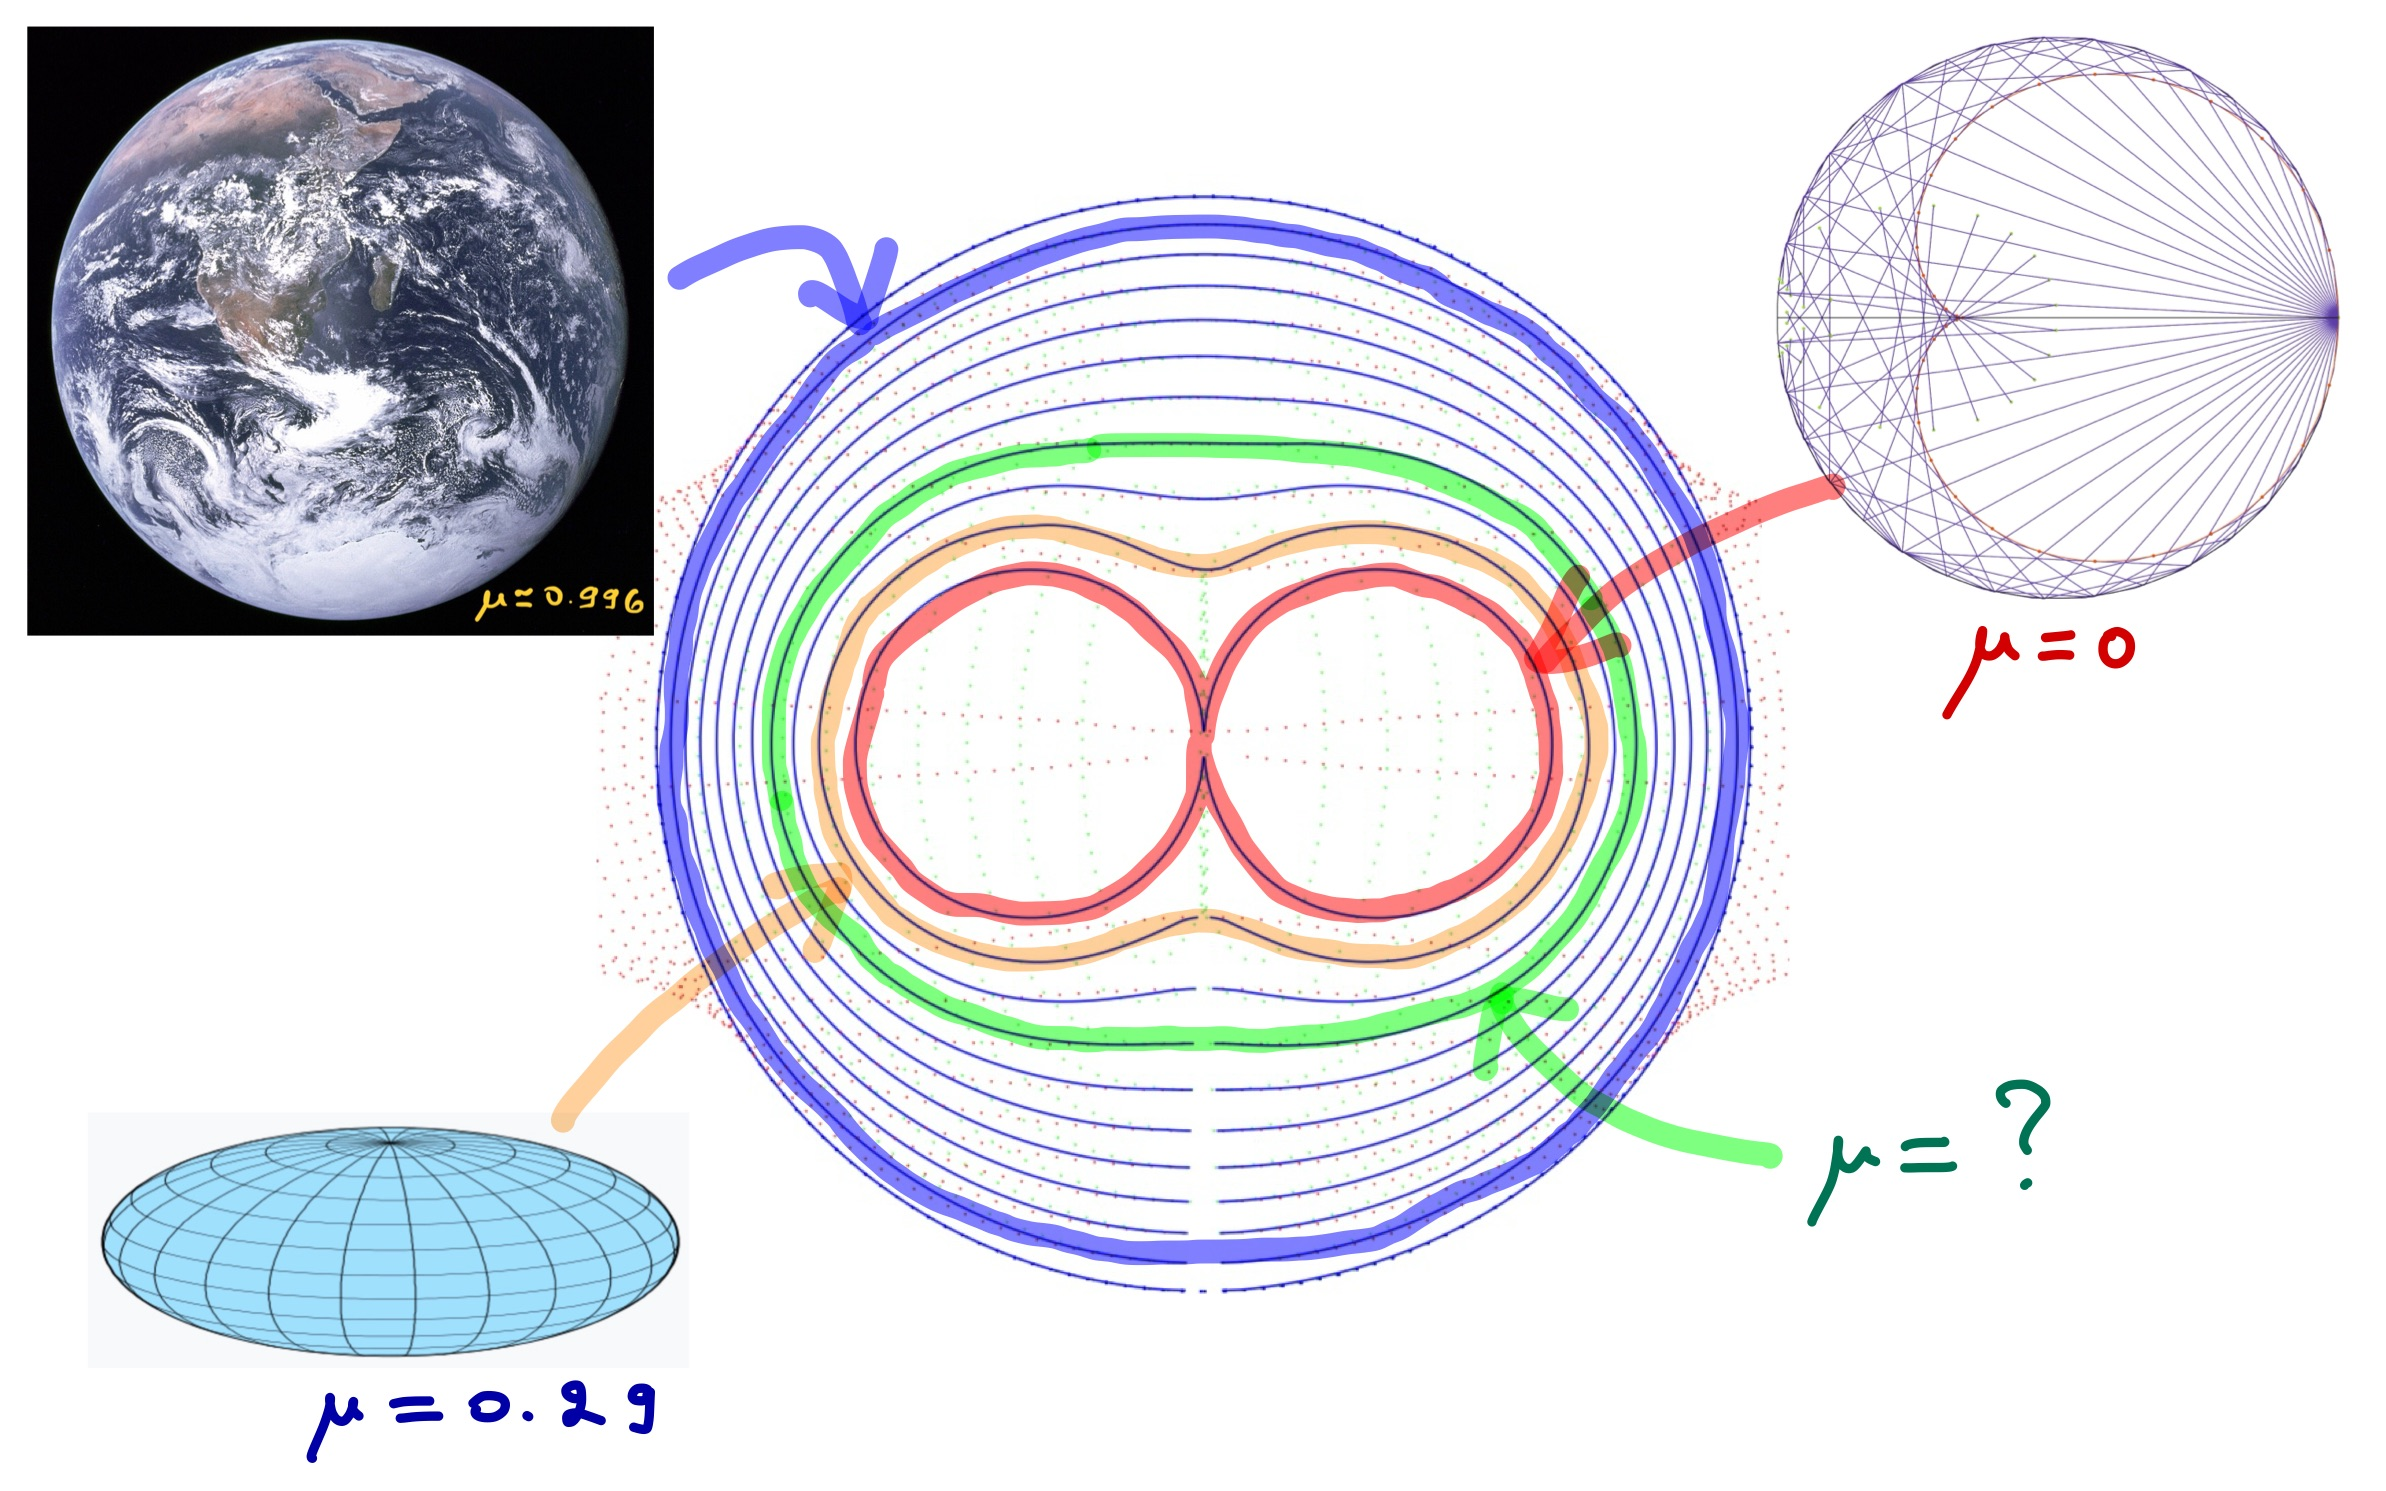
\includegraphics[height=7.0cm]{oblat4}

\end{frame}

% Un calcul
\begin{frame}
\frametitle{\bf Un calcul}
 
\centering 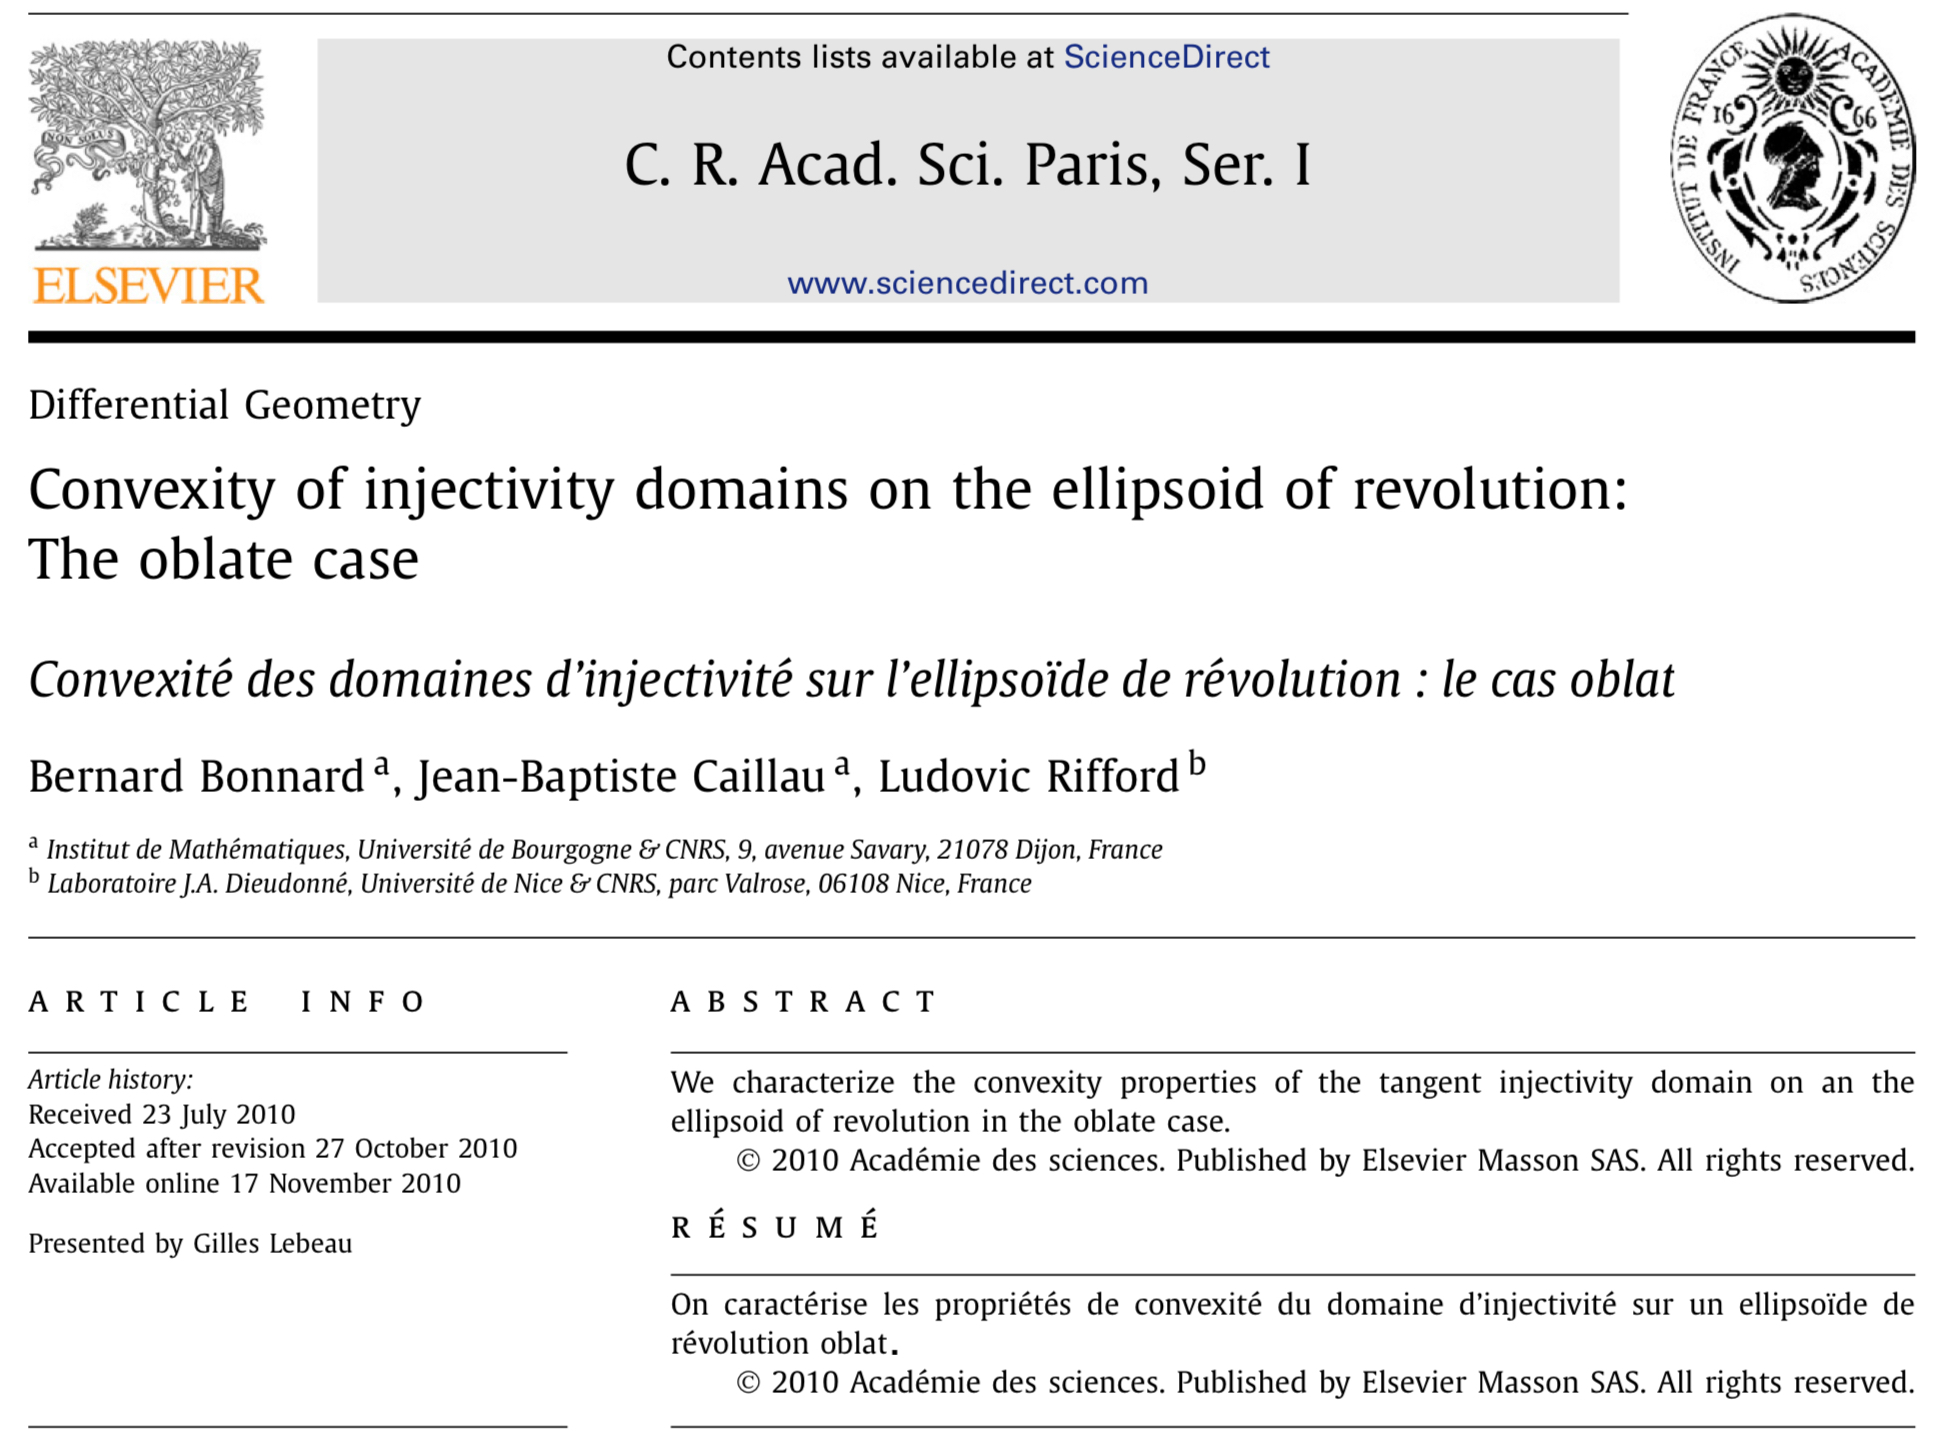
\includegraphics[height=7.0cm]{cras1}

\end{frame}

% Un calcul
\begin{frame}
\frametitle{\bf Un calcul}
 
\centering 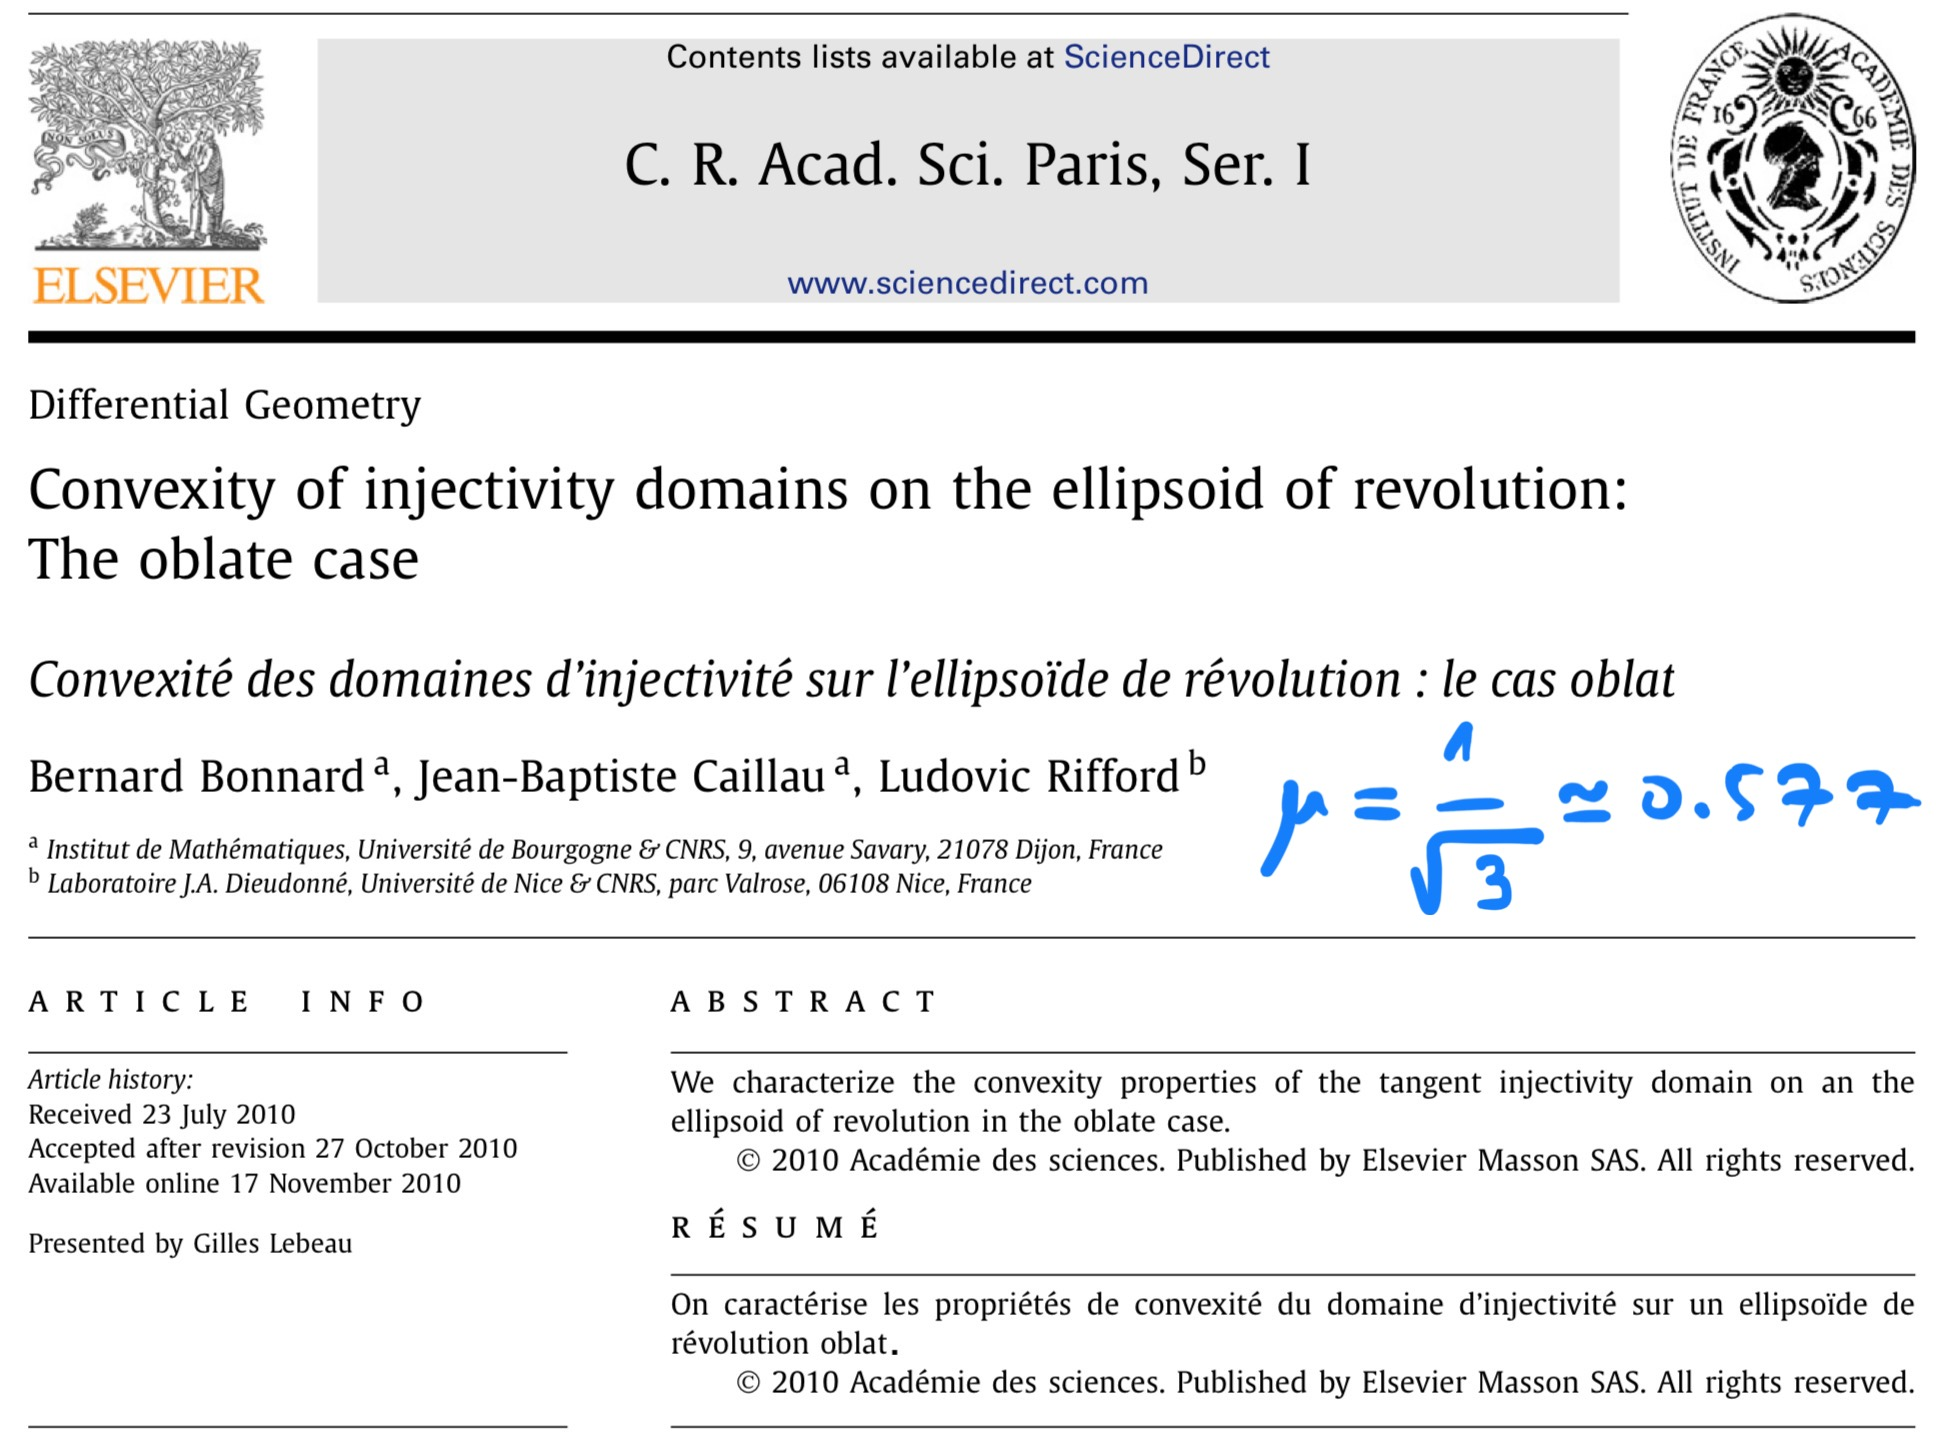
\includegraphics[height=7.0cm]{cras2}

\end{frame}

% D'une fleur \`a l'autre... contin\^ument
\begin{frame}
\frametitle{\bf D'une fleur \`a l'autre... contin\^ument}
 
\centering 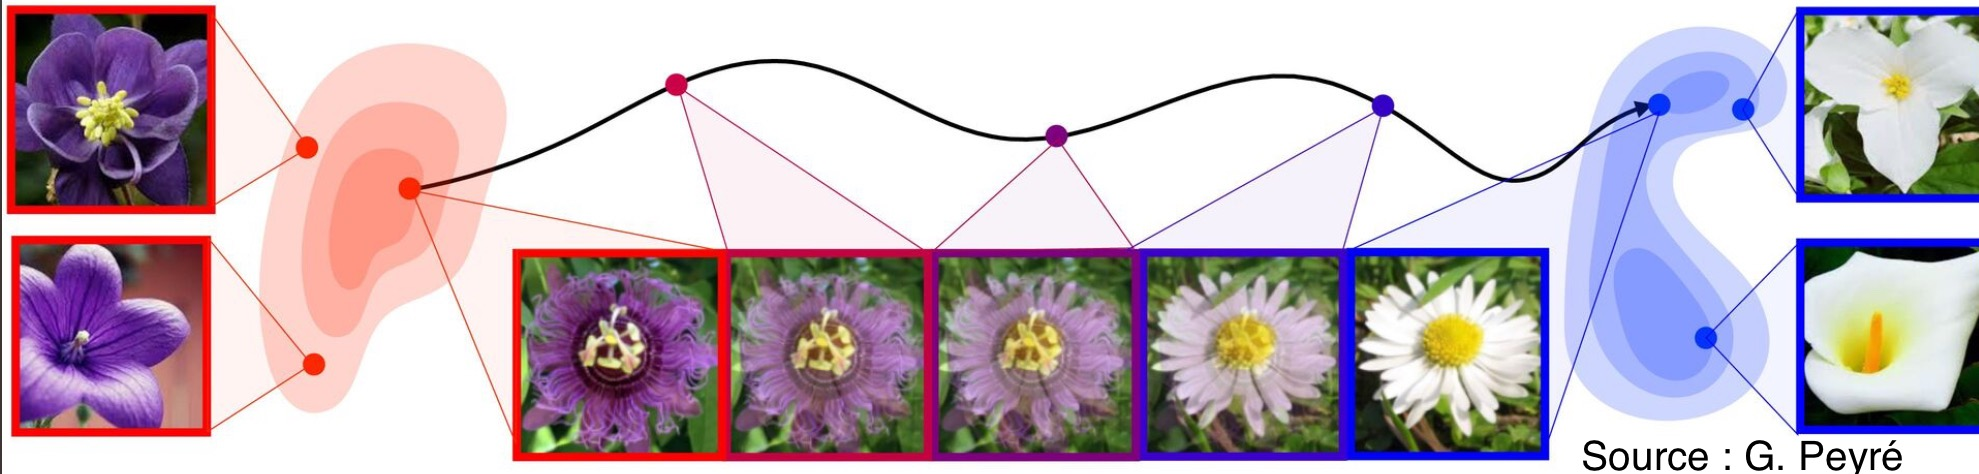
\includegraphics[height=2.8cm]{fleur}

\end{frame}

% Disparition (continue)
\begin{frame}
\frametitle{\bf Disparition (continue)}
 
\centering 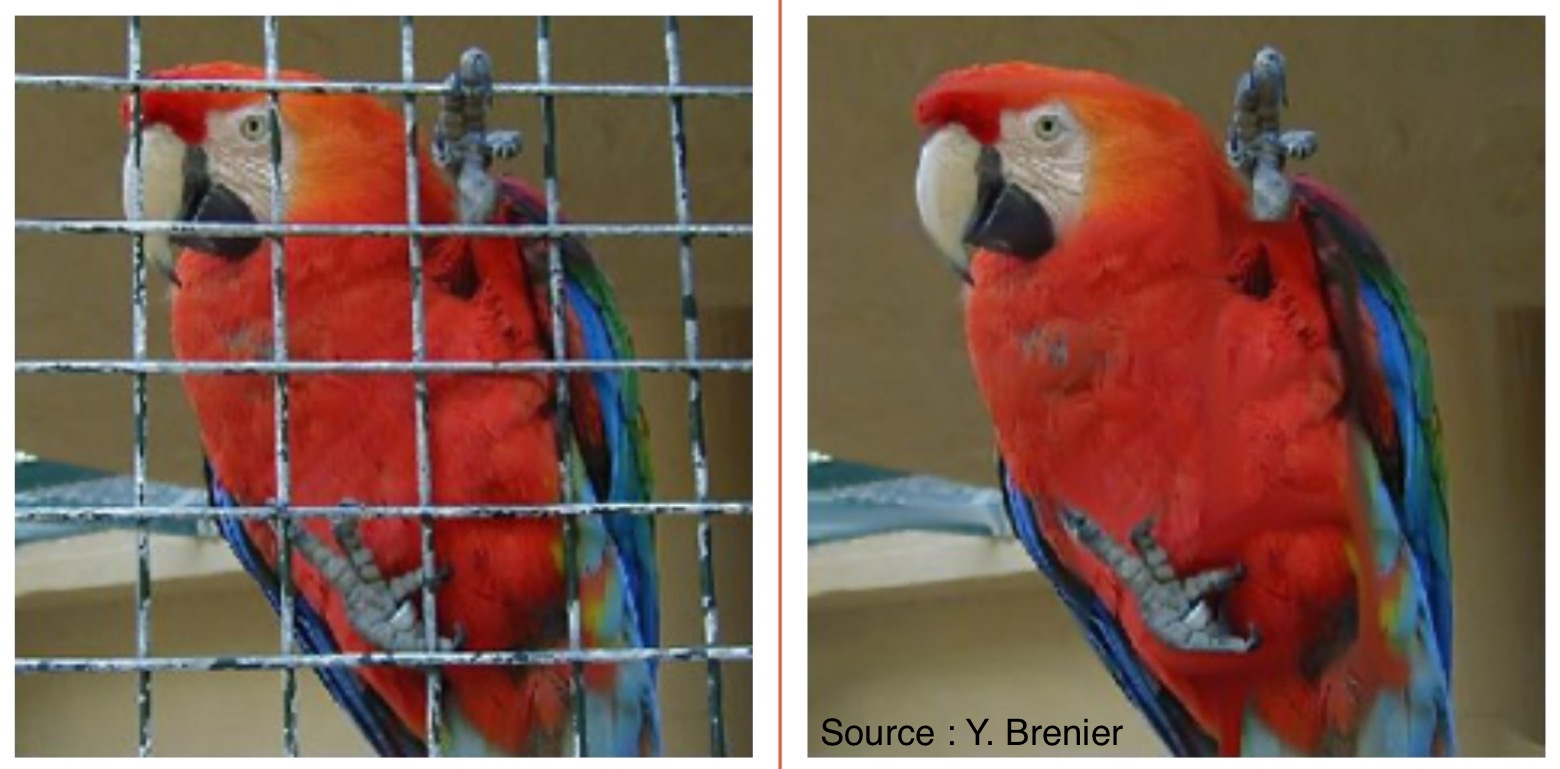
\includegraphics[height=5.0cm]{parrot}

\end{frame}

% Conclusion
\begin{frame}
\frametitle{\bf Conclusion}

\begin{quote}
"\`A partir d'applications tr\`es simples en apparence, il fait na\^\i tre l'id\'ee de th\'eories abstraites dont on n'avoit pas encore le besoin [et dirige] vers les th\'eories [les] travaux des g\'eom\`etres, et leur [ouvre] une carri\`ere nouvelle." Condorcet (1743--1794)
\end{quote}
 
\begin{quote}
"Il n'y a pas des probl\`emes qu'on se pose, il y a des probl\`emes qui se posent. Il n'y a pas de probl\`emes r\'esolus, il y a seulement des probl\`emes plus ou moins r\'esolus". H. Poincar\'e (1854--1912)
\end{quote}

\centering 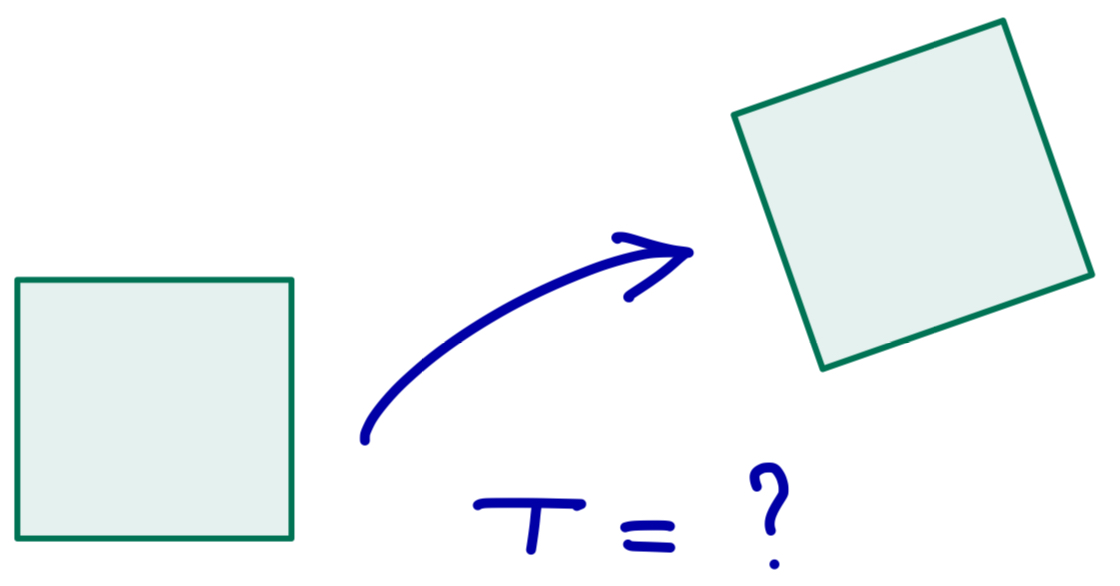
\includegraphics[height=4.0cm]{carre}

\end{frame}

% R\'ef\'erences
\begin{frame}
\frametitle{\bf R\'ef\'erences}
 
\begin{itemize}
  \item Brenier, Y.; Vi\'eville, T. \emph{La brouette de Monge ou le transport optimal.} Images des Math\'ematiques, CNRS, 2010
  \item Ghys, E. \emph{Gaspard Monge, math\'ematicien de la R\'evolution.} Images des Math\'ematiques, CNRS, 2010
  \item Peyr\'e, G. Homepage
\end{itemize}

\end{frame}

% Vers la recherche
\begin{frame}
\frametitle{\bf Vers la recherche}

\centering 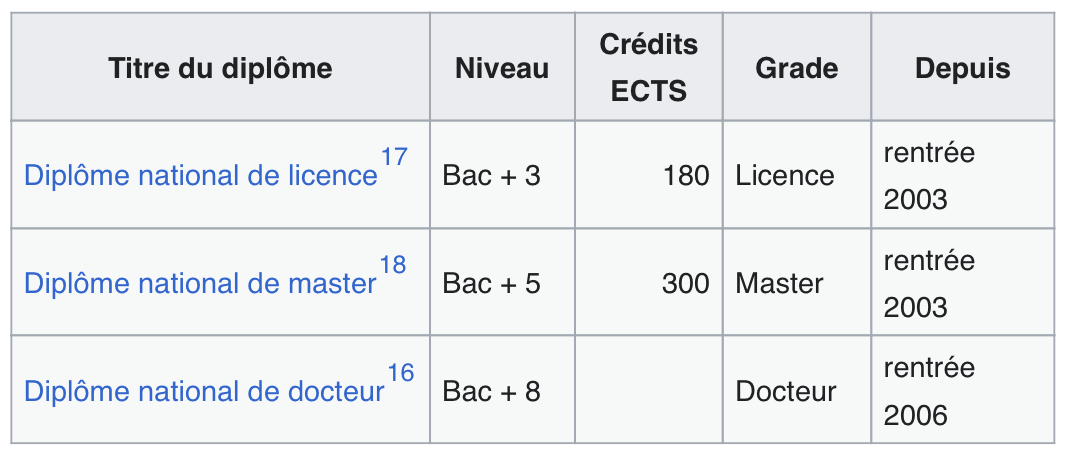
\includegraphics[height=4.0cm]{lmd}
 
\begin{itemize}
  \item Ma\^itre de conf\'erences / Charg\'e de recherche 
  \item HDR $\rightarrow$ Professeur / Directeur de recherche
\end{itemize}

\end{frame}

\end{document}

%% - math applis / fonda : obsolète, plutôt pas pertinent
%% - Massena : 1758-1817
%% - discret -> continu, plat -> surface avec courbure, [relaxation Kanto / mesure]
%% - caustique : kaio (je brule)
%% https://images-des-maths.pages.math.cnrs.fr/freeze/Gaspard-Monge,1094.html
%% https://images-des-maths.pages.math.cnrs.fr/freeze/Gaspard-Monge.html
%% https://images-des-maths.pages.math.cnrs.fr/freeze/La-brouette-de-Monge-ou-le-transport-optimal.html